\begin{refsection}
	\chapter[What Type of Finance Matters for Growth? BMA Evidence]{What Aspect of Financial Intermediation Matters for Growth? Bayesian Model Averaging Evidence}
\label{ch2}
\blfootnote{This chapter was co-authored with Iftekhar Hasan and Roman Horv\'{a}th and large part of it published in \emph{The World Bank Economic Review} as \emph{What Type of Finance Matters for Growth? Bayesian Model Averaging Evidence}. We thank Martin Feldkircher and seminar participants at 19th ICMAIF conference (Rethymno, Greece), 32nd International Symposium on Money, Banking and Finance (Nice, France) and 1st World Congress for Comparative Economics (Rome, Italy) for helpful comments. The views expressed here are those of the authors and not necessarily those of the Czech Ministry of Finance or Bank of Finland.}

\begin{quote}
\begin{center}\textbf{Abstract}\end{center}
	We examine the effect of finance on long-term economic growth using Bayesian model averaging to address model uncertainty in cross-country growth regressions. The literature largely focuses on financial indicators that assess the financial depth of banks and stock markets. We examine these indicators jointly with newly developed indicators that assess the stability and efficiency of financial markets. Once we subject the finance-growth regressions to model uncertainty, our results suggest that commonly used indicators of financial development are not robustly related to long-term growth. However, the findings from our global sample indicate that one newly developed indicator -- the efficiency of financial intermediaries -- is robustly related to long-term growth.     
	\end{quote}

\clearpage
\section{Introduction}
\label{ch2sec:intro}
Numerous studies investigate the effect of financial development on economic growth and predominantly conclude that there is a positive causal relationship between the two \parencite{KingLevine1993a, LevineZervos1998, AtjeJovanovich1993}. Nevertheless, some opposing views hold that the financial sector removes scarce resources from the rest of the economy \parencite{Tobin1984,Boltonetal2011} and encourages to greater exposure and vulnerability to crises, thus severely burdening the real sector during periods of instability \parencite{Kindelberger1978,Minsky1991,Stiglitz2000}. The effect of financial development on growth drew greater attention again because of the financial crisis that began in 2007-2008. Moreover, conclusions referring to diminishing and eventually negative returns from financial development have become increasingly common in the literature \parencite{Arcandetal2012,CecchettiKharroubi2012,LawSingh2014}. This highlights the importance of the financial sector for the functioning of the economy and has provoked extensive debate among policymakers. 

This paper evaluates the finance-growth nexus but differs from existing research in two main respects. First, it employs \ac{BMA} to overcome certain drawbacks of previous research approaches. \ac{BMA} is well grounded in statistical theory \parencite{Rafteryetal1997} and addresses the inherent regression model uncertainty, which is quite high in cross-country growth regressions \parencite{Fernandezetal2001, SalaiMartinetal2004, Durlaufetal2008}. The control variables in finance-growth regressions are often selected in a somewhat \textit{ad hoc} manner with reference to certain relevant theories while ignoring other relevant theories. 

\ac{BMA} essentially allows us to control for dozens of potentially relevant determinants of growth within a unifying framework. The variety of theories of economic growth has given rise to a large number of determinants and resulted in substantial uncertainty concerning the true growth model. In essence, the \ac{BMA} procedure estimates different combinations of explanatory variables and subsequently weights the coefficients using various measures of model fit. As a consequence, \ac{BMA} also conveniently limits concerns regarding omitted variable bias and its adverse consequences of inconsistently estimated coefficients, an issue that is typically abstracted from in the empirical work on finance and growth. \ac{BMA} is capable of evaluating numerous possible regressors and estimating their \ac{PIP}, i.e., the probability that they are relevant in explaining the dependent variable, in addition to the weighted mean and variance of their corresponding coefficients. While model averaging has become standard in the empirical growth literature \parencite{SalaiMartinetal2004, Durlaufetal2008}, it has not been applied to study the finance--growth nexus.  

Second, we differ from previous research by examining additional financial indicators to appreciate the multidimensionality of financial systems. Importantly, previous research, including recent studies implying that excessive financial development harms growth \parencite{Arcandetal2012,CecchettiKharroubi2012,LawSingh2014}, largely focuses on measures of the depth of financial development such as the credit to GDP ratio. We depart from existing literature in jointly examining whether the depth, stability or efficiency of financial markets (or all of them) is crucial for long-term growth. In doing so, we can unify and re-examine previous studies on the finance-growth nexus that show that a) financial development is conducive to growth, b) excessive financial development is not, and c) financial instability has negative consequences for growth.

The theoretical concepts regarding the functions of the financial industry are difficult to operationalize in empirical research, and there is no universal consensus regarding the measurement of financial development \parencite{KingLevine1993a}. Although measuring financial development is complex, researchers typically consider only those variables capturing financial depth, such as the credit to GDP ratio or stock market capitalization, to assess the degree of financial development. Financial indicators assessing the degree of financial access, financial stability or the efficiency of the financial industry have largely been ignored in cross-country studies due to data limitations. The newly developed \ac{GFDD} represents a significant improvement in this respect and provides a comprehensive set of financial indicators that reflect various functions and characteristics of the financial sector. In addition to financial depth, the \ac{GFDD} provides measures of the efficiency and stability of and access to financial markets. Although data availability remains somewhat limited, we extend the existing literature by including these additional dimensions of the financial sector in our regression analysis to more completely evaluate the effect of finance on growth. Specifically, the indicators we use represent the depth, stability, and efficiency of the banking sector and stock markets as defined by \textcite{Cihaketal2013}.\footnote{We did not include financial access indicators because of data unavailability. In our sample, the data on the proxy variable recommended for financial access by \textcite{Cihaketal2013}, bank accounts per 1,000 adults, are missing for 36 out of 60 countries. Including financial access in the analysis would therefore severely limit our cross-section of countries resulting in the non-negligible loss in the degrees of freedom. Nevertheless, we have examined alternative (less than ideal) financial access indicators from the \ac{GFDD} database (bank branches per 100,000 adults and ATMs per 100,000 adults), which are available for almost all countries in our sample. However, we fail to find these indicators to be decisive for the long-term growth.} In addition to the \ac{GFDD}, we employ the widely used dataset on the determinants of long-term growth developed by \textcite{Fernandezetal2001}, which encompasses over 40 explanatory variables capturing various economic, political, geographical, and institutional indicators. 

While it is commonly assumed that causality goes from financial development to economic growth, some scholars argue that a growing financial sector merely follows the increasing needs of the real economy or may be determined simultaneously with growth due to other factors. The quantitative survey of the finance and growth literature by \textcite{Valickovaetal2014}, for example, indicates that those studies ignoring endogeneity are more likely to report a stronger positive effect of financial development on growth. Although it is likely that a part of endogeneity in finance--growth nexus can be addressed by model averaging procedure (reducing omitted variable bias), we also examine the robustness of our results through specifications that employ the lagged explanatory variables. To the best of our knowledge, this is the first study to combine various characteristics of the financial sector, a rich dataset on growth, and an approach that addresses model uncertainty and endogeneity. As a result, our study addresses two main issues in finance--growth literature: 1) causality issues and 2) measurement of financial development.

Using data on real economic growth in 60 countries between 1960 and 2011, we find that bank efficiency is robustly related to long-term growth and exhibits very high \ac{PIP}. This finding corresponds to the predictions of theoretical model by \textcite{Pagano1993}, who shows that the efficiency of financial intermediaries is crucial for funneling savings to investment and therefore, for increasing real growth. The relevance of traditional variables, such as credit provided to the private sector or stock market capitalization, is weaker. In addition, we also fail to find a non-linear effect of financial development on growth.  Our results are robust to a series of checks such as employing a different sample period, different parameter priors or addressing endogeneity. Therefore, our results highlight that the approach to measuring financial development is crucial for the estimated effect of finance on growth. Our policy implication is that those managing the current worldwide wave of regulatory changes in the financial industry should not underestimate the importance of the efficiency of financial intermediaries for long-term growth.

The chapter is structured as follows. Section \ref{ch2sec:litsurvey} provides a literature review on finance and growth. Section \ref{ch2sec:data} presents the data. We describe Bayesian model averaging in Section \ref{ch2sec:BMA}. We provide the regression results in Section \ref{ch2sec:Results}. The conclusions are presented in Section \ref{ch2sec:conclusions}. An appendix with additional results follows. 
%
%
% 
%
%
\section{Empirical Literature on Finance and Growth}
\label{ch2sec:litsurvey}

We briefly survey the empirical literature on the effect of financial development on growth. In addition, we discuss certain issues regarding the measurement of financial development. We refer readers to \textcite{Levine2005}, \textcite{Ang2008} and \textcite{Valickovaetal2014} for more comprehensive surveys of this literature.\footnote{There is also literature on the determinants of financial development, see \textcite{Ang2013}, and \textcite{angkumar}.}

\subsection{Empirical Evidence}

Focusing on the period between 1960 and 1989, \textcite{KingLevine1993a} show how the initial levels of various financial indicators, such as the liabilities to the financial sector, bank ratios, credit to nonfinancial private sector/total domestic credit, and credit to the private sector to GDP, explain the real growth of GDP per capita, capital accumulation, and efficiency of capital utilization in the following period. \textcite{AtjeJovanovich1993} examine the stock market's effects on economic growth and find that more active stock markets induce growth. The conclusion regarding stock market activity is subsequently confirmed by \textcite{LevineZervos1998}. In addition to providing evidence on stock market effects, \textcite{LevineZervos1998} simultaneously control for banking sector development by including credit to the private sector. Interestingly, both the banking sector and stock markets are significant in fostering growth. This leads the authors to conclude that each of the sectors has a different function in the economy and a different financial function. Furthermore, they add that the mere size of the stock market as measured by total capitalization is irrelevant to growth and that the relevant factor is the activity of the stock market. Nevertheless, this link may be an outcome of an unobserved third factor that stimulates both trading activity and economic growth. For instance, information regarding new technology may spur trading activity due to conflicting opinions on the future benefits of the innovation. The subsequent economic growth is a result of technological advancement rather than greater trading volumes \parencite{Levine2005}. This is one of the reasons why we apply the \ac{BMA}, which is designed to address these issues.

\textcite{RajanZingales1998} initiate the research on the finance-growth nexus using industry-level data. They show that more developed financial markets decrease firms' cost of external capital. They also find evidence that industries that are relatively more dependent on external finance grow faster in countries with better developed financial intermediaries. Building on this methodology, \textcite{ClaessensLaeven2005} arrive at a similar conclusion using measures of bank competitiveness. They find that more competitive banking systems benefit financially dependent industries. Next, \textcite{Becketal2005} show that industries typically composed of small firms enjoy relatively superior growth rates in countries with developed financial sectors. This is consistent with theory positing that financial development is a crucial factor in alleviating financial constraints. Also, \textcite{Hasanetal2009} examine the effect of financial development on regional growth in Europe and find that the efficiency of financial intermediaries (measured by bank efficiency) is substantially more important for growth than financial depth (measured by outstanding credit). \textcite{Bergeretal2004} also provide international evidence on the importance of bank efficiency for growth. Similarly, using German data, \textcite{KoetterWedow2010} find that bank efficiency is positively related to growth. \textcite{JayaratneStrahan1996} report that the relaxation of bank branch restrictions in the United States improves growth. Interestingly, they find that the relaxation of restrictions does not increase the volume of bank lending but improves loan quality. In addition, \textcite{CetorelliStraha2006} extensively examine the mechanism how financial development affect growth and find that more competition among local U.S. banks improves firms' performance. 

Panel and time-series analyses predominantly claim that the relationship goes from financial development to growth rather than in the reverse direction, essentially moderating endogeneity concerns.  \textcite{ChristopoulosTsionas2004}, \textcite{Finketal2003} and \textcite{PeiaRoszbach2015} observe positive long-run growth effects of financial development using cointegration techniques. \textcite{ChristopoulosTsionas2004} argue in favor of long-run causality from financial development to growth and dismisses the backward channel. \textcite{Finketal2003} is one of the few papers investigating the relationship by considering private bond markets. \textcite{PeiaRoszbach2015} investigate the causality of the finance-growth relationship and demonstrate that the causality depends on the measurement employed and the level of financial development. Recently, \textcite{Thumrongvitetal2013} revisit the question and compare the impact of bond markets while also accounting for the role of the banking sector. They report that the importance of bank credit in determining growth declines as alternative debt financing options become increasingly available. Although studies positing ``finance-lead'' growth prevail, there are opposing views that stress finance's irrelevance in this respect. \textcite{Garretsenetal2004}, for example, document that the causal link reported by \textcite{RajanZingales1998} disappears after accounting for societal and legal factors. It may be that the development of financial markets simply follows growth, reflecting the needs of a more developed economy. Ultimately, accounting for time- and country-specific effects does not entirely eliminate the caveats applicable to such analyses. Time coverage is often short, and utilizing more frequent observations, such as quarterly data, does not properly address hypotheses concerning the long-term nature of the relationship \parencite{Ang2008}. 

Researchers have devoted greater attention to the finance and growth literature following the economic crisis of 2007-2008. They raise questions regarding possible non-linearities in the relationship between finance and growth, specifically, whether excessive financial development is harmful to growth. \textcite{RousseauWachtel2011} report that a positive correlation between the development of the financial sector and economic growth is typical for the period before 1990. The effect diminishes when subsequent years are considered. Additional studies report evidence of an inverted U-shaped relationship suggesting financial development is conducive to growth only up to a certain threshold. Thereafter, it acts as a drag on economic growth \parencite{CecchettiKharroubi2012,Arcandetal2012,LawSingh2014}. Some research advances explanations to justify these findings. One is the comparatively large amount of credit going to households in the later stages of financial development. These loans generally tend to be less productive than loans to enterprises \parencite{Becketal2012}. \textcite{CecchettiKharroubi2013} emphasize that a larger financial sector leads to lower total factor productivity through relatively larger benefits for high-collateral/low-productivity projects, primarily in construction. Other lines of reasoning rely on Tobin's early work discussing how finance lures talent from other sectors \parencite{Boltonetal2011,CecchettiKharroubi2012,Kneer2013}. \textcite{Yilmazkuday} shows that growth enhancing effect of finance depends on a number of factors such as price stability, economic development or trade openness. Overall, these recent empirical studies find that the growth-enhancing effects of financial development are not guaranteed and suggest that the relationship is more complex than originally thought.

\subsection{Measurement of Financial Development}
\textcite{Levine2005} argues that it is difficult to link empirical and theoretical research on finance and growth. Concepts such as information asymmetry, improved corporate governance, risk management, pooling savings, and easing exchange are in reality difficult to measure accurately.

The most common indicators of financial development address financial depth, primarily because of their widespread availability. Conventional variables used as proxies for the depth of the financial sector are total liquid liabilities of the financial sector, credit to the private sector, and various measures of monetary aggregates. The aforementioned variables depict the development of the banking sector, in stock market studies, broadly employed proxies include the ratio of total market capitalization to GDP, the total value traded to GDP (stock market activity ratio), and the total value traded to the total value of listed shares (turnover ratio).  

The extent to which these traditional measurements reflect the ability of financial intermediaries to serve the functions assigned to them in theory remains unclear. For instance, \textcite{Cihaketal2013} illustrate that private bond market capitalization represents a substantial share of the total securities market capitalization within a country. However, when addressing the question of depth, private bond markets are often ignored. In addition, total credit data do not include trade credit, where firms \textit{de facto} act as financial intermediaries \parencite{PetersenRajan1997}. In addition, \textcite{Levine2005} notes that this factor may be particularly important in countries with poor legal environments or overly regulated financial systems. Ultimately, there is no general consensus among researchers regarding the appropriate approach to measure financial development. Generally, studies consider several potential indicators to assess the robustness of their results, but these indicators are typically only proxies for the level of financial depth \parencite{Valickovaetal2014}.

Finally, some financial development measures such as the (rarely used) bank efficiency can be conceptually much more closely related to the theory \parencite{Pagano1993} than the traditional quantity measures such as the volume of credit granted. Bank efficiency is also less likely to be prone to causality issues because technical efficiency of banks respond less to the business cycle in comparison to, for example, the volume of credit \parencite{KoetterWedow2010}.

\section{Data}
\label{ch2sec:data}
We use the dataset from a seminal paper on long-term economic growth determinants and \ac{BMA} by \textcite{Fernandezetal2001}. The dataset contains 41 explanatory variables that might be important for growth in 72 countries. We update the dependent variable (average real economic growth per capita in 1960-2011). The regressors in the dataset comprise various measures of economic, political, geographic, demographic, social, and cultural factors. As many of these factors may be determined simultaneously with growth, the regressors typically come from 1960 or even before to alleviate endogeneity concerns. We describe this dataset in greater detail in the appendix.

To this dataset, we add selected financial indicators from the World Bank's \ac{GFDD} (September 2013 version), which collects information on various aspects of financial sectors around the globe. \textcite{Cihaketal2013} describe this dataset's content in detail and offer a 4x2 dimensional classification of financial indicators that reflects their utility in representing the depth, breadth, efficiency, and stability (4) of both the banking sector and the stock market (2). We choose to employ several indicators for which the database provides the richest data. Specifically, we select five different indicators representing various aspects of the financial system:

\begin{itemize}
	\item \textbf{Private sector credit to GDP:} domestic private credit to the real sector to GDP; a measure of the depth of the banking sector.
	\item \textbf{Stock market capitalization to GDP:} value of listed shares to GDP; a measure of the depth of stock markets.
	\item \textbf{Net interest margin:} accounting value of banks' net interest revenue as a share of average interest-bearing assets; a measure of the efficiency of the banking sector.
	\item \textbf{Stock market turnover ratio:} stock market value traded to total market capitalization; a measure of the efficiency of stock markets.
	\item \textbf{Bank Z-score:} return on banks' assets plus the ratio of banks' equity and assets, divided by the standard deviation of the return on assets $\left(\frac{ROA + \frac{equity}{assets}}{sd(ROA)}\right)$; a measure of the stability of the banking sector.
\end{itemize} 
%
The aforementioned dimensional distinction allows us to differentiate and compare the effects of the banking sector and the stock market on economic growth. In addition, unlike the previous literature, we simultaneously examine whether the depth, efficiency and stability of a financial system are important for growth. 

The time and cross-country coverage of financial variables varies. Private credit to the real sector is available for the majority of the countries in the dataset since 1960. However, the remaining variables are typically available only from the 1980s onward. We average the indicator values corresponding to a selected period (i.e., 1960-2011) and to their data availability. This is a standard procedure in estimating empirical long-term growth models, despite the risk of introducing endogeneity into the model and information loss introduced by averaging over extended time periods. The benefit of averaging is a focus on long-term trends while abstracting from short-term fluctuations. But in our robustness checks, we also use the initial values of financial indicators instead of their average. Given the data availability and the construction of the dataset, all the financial variables could be endogenous. We address endogeneity concerns through our \ac{BMA} approach using lagged variables. Table \ref{tab:descstat} presents descriptive statistics on the individual financial indicators. Overall, the combined dataset of \textcite{Fernandezetal2001} and private credit and new financial indicators leads to 68 and 60 observations, respectively.

\begin{table}[!ht]
	\caption{Descriptive statistics, financial indicators}
	\label{tab:descstat}
	\centering
	\begin{tabular}{lrrrrr}
		\toprule
		& Min & Max & Mean & Std.dev \\ 
		\midrule
		Net interest margin 		& 0.59 & 13.31 & 4.52 & 3.25 \\ 
		Bank Z-score				& -1.61 & 42.35 & 15.00 & 9.62 \\ 
		Private credit 			& 5.16 & 146.66 & 46.58 & 35.29 \\ 
		Market capitalization 	& 0.67 & 303.77 & 51.28 & 52.98 \\ 
		Market turnover 			& 0.96 & 197.50 & 48.22 & 47.13 \\ 
		\bottomrule
		
	\end{tabular}
\end{table}

\section{Bayesian Model Averaging}
\label{ch2sec:BMA}
To illustrate the application of BMA, we begin with a traditional linear model structure:
%
% OLS notation
\begin{equation}\label{ch2eq:OLS}
	y = \alpha + X\beta+ \varepsilon \qquad \varepsilon  \sim\ N(0, \sigma^{2}I)
\end{equation}
%
where $y$ is a dependent variable, $\alpha$ is a constant, $X$ is the matrix of explanatory variables, $\beta$ represents the corresponding coefficients, and $\varepsilon$ is a vector of normally distributed IID error terms with variance $\sigma^{2}$. In many applications, the list of potentially relevant regressors can be large. In the typical case in which the true regression model is unknown, its construction often begins by including all the variables in the model. However, this strategy is likely to yield imprecise estimates, as the large number of regressors inflates standard errors. Empirical research typically addresses this issue by sequentially eliminating the least significant explanatory variables on the basis of statistical tests to arrive at the single best model with all the irrelevant regressors omitted.

The process described above entails the risk of the researcher retaining an irrelevant variable or dropping an important variable. \textcite{Koop2003} emphasizes that the probability of making such mistakes increases rapidly with the number of sequences performed. The various iteration paths may also lead to different regression model specifications. In addition, even if we assume that this procedure identifies the 'best' model, it is rarely acceptable to present only the results from the single 'best' model and disregard the results of 'second-best' models. In summary, then, this model-selection approach ignores the model uncertainty that the researcher faces when she or he defines the model. \ac{BMA} allows the researcher to account for such uncertainty and presents a rigorous method for treating multiple models.

\ac{BMA} considers all possible combinations of $X$ from equation \ref{ch2eq:OLS} and takes a weighted average of the coefficients (see also the remarks on the \ac{MCMC} sampler below). The substructure of the model can be captured as follows:
%
% submodel structure
\begin{equation}\label{ch2eq:OLSsub}
	y = \alpha_{i} + X_{i}\beta_{i}+ \varepsilon \qquad \varepsilon  \sim\ N(0, \sigma^{2}I)
\end{equation}
%
Here, $X_{i}$ is a subset of $X$ and $\alpha_{i} $ and $ \beta_{i}$ are the corresponding coefficients. Assuming that the total number of possible explanatory variables is $K$, the total number of models is equal to $2^{K}$ and $i \in [1,2^{K}]$. 
%%
%%
%%

Researchers are interested in describing coefficients based on observed data. It follows from Bayes' rule that
%
% Bayes' rule with 'model' notation
\begin{equation}\label{ch2eq:BRmodel}
	p(\beta \vert y,X) = \frac{p(y,X\vert \beta)p(\beta)}{p(y,X)}
\end{equation}
where $p(\beta \vert y, X)$ is the posterior density, $p(y, X\vert \beta)$ is the marginal likelihood (ML), also known as the data generating process, $p(\beta)$ is the prior density, and $p(y,X)$ is the probability of the data. In the \ac{BMA}, we essentially compare numerous different models $M_{1},...,M_{i}$.  Assuming $K$ possible regressors as discussed above, we have $M_{1},...,M_{i}$, where $i \in [1,2^{K}]$. Given the Bayesian logic whereby we formally define the model using a likelihood function and a prior density, $M_{i}$ depends on the parameters $\beta_{i}$, and their posterior probability can be derived as follows:
\begin{equation}\label{ch2eq:BROM}
	p(\beta_{i} \vert M_{i},y,X) = \frac{p(y\vert \beta_{i},M_{i},X)p(\beta_{i}\vert M_{i})}{p(y \vert M_{i},X)}
\end{equation}
The following subsections describe the averaging principle of \ac{BMA} and individual components of equation \ref{ch2eq:BROM}.
%
%%
\subsection{Posterior Model Probability}
%%
%
The \ac{PMP} is fundamental to the \ac{BMA} framework, as it provides the weights for averaging model coefficients across submodels. \ac{PMP} also arises from Bayes' theorem:

\begin{equation}\label{ch2eq:PMPmain}
	p(M_{i} \vert y,X) = \frac{p(y\vert M_{i},X)p(M_{i})}{p(y \vert X)}
\end{equation}

where $p(y\vert M_{i},X)$ is the \ac{ML} of the model (i.e., the probability of the data given the model $M_{i}$), $p(M_{i})$ is the prior model probability, and $p(y\vert X)$ is the integrated likelihood. The term in the denominator is typically disregarded, as it is constant across all models under consideration. The PMP is then directly proportional to \ac{ML} and the prior probability. A popular practice is to set the prior probability $p(M_{i} \propto 1)$ to reflect the lack of knowledge regarding the true model.
% Proportionality of PMP
\begin{equation}
	p(M_{i}\vert y,X) \propto p(y\vert M_{i},X)p(M_{i})
\end{equation}
%
We discuss the calculation of \ac{ML} in detail in Subsection \ref{ch2sec:ML}. The model prior needs to be elicited by the researcher and reflects the initial beliefs before inspecting the data. 
%
\subsection{Posterior Mean}
Point estimates of the model parameters are often the focus of research, and it is possible to derive them within the Bayesian framework. \textcite{Zeugner2011} and \textcite{MoralBenito2012} assert that the weighted posterior distribution of any statistic (most notably the $\beta$ coefficients) is obtained using the following:
%
%% Posterior distribution of the coefficients
\begin{equation}\label{ch2eq:parest}
	p(\beta \vert y, X) = \sum_{i=1}^{2^{K}} p(\beta_{i} \vert M_{i},y,X)p(M_{i} \vert y,X)
\end{equation}

where $p(M_{i} \vert y, X)$ is the \ac{PMP} of the corresponding model $M_{i}$ from equation \ref{ch2eq:PMPmain}. The point estimates can be acquired by taking expectations across the equation:

\begin{equation}\label{ch2eq:pointparest}
	E(\beta \vert y, X) = \sum_{i=1}^{2^{K}} E(\beta_{i} \vert M_{i},y,X)p(M_{i} \vert y,X)
\end{equation}

Here, $E(\beta \vert y, X)$ is the averaged coefficient and $E(\beta \vert M_{i},y,X)$ is the estimate of the $\beta_{i}$ coefficients from model $M_{i}$. The posterior distribution of the coefficients is dependent on the choice of the prior $g$. \textcite{Zeugner2011} expresses the expected value of the parameter in $M_{i}$ as follows:
\begin{equation}\label{ch2eq:postdist}
	E(\beta_{i} \vert y,X,g,M_{i}) = \frac{g}{1+g}\hat{\beta_{i}}
\end{equation}
with $\hat{\beta_{i}}$ representing the standard \ac{OLS} estimate.

\subsection{Posterior Variance}
\textcite{MoralBenito2012} presents a formula for variance corresponding to the expected values of coefficients derived in the previous section:
\begin{equation}\label{ch2eq:postvar}
	\begin{aligned}
		Var(\beta \vert y, X) &= \sum_{i=1}^{2^{K}} p(M_{i} \vert y,X)Var(\beta_{i} \vert M_{i},y,X) + \\ 
		&+\sum_{i=1}^{2^{K}}p(M_{i} \vert y,X){(E(\beta_{i}\vert M_{i},y,X)-E(\beta \vert y, X))}^{2}
	\end{aligned}
\end{equation}
The variance consists of the weighted average of variance estimates across different regression models $Var(\beta_{i} \vert M_{i},y,X)$ and the weighted variance across different models captured in the second component ${{E(\beta_{i}\vert  M_{i},y,X)}-{E(\beta \vert y,X))}}^{2}$. $E(\beta \vert y,X)$ is the posterior mean from equation \ref{ch2eq:pointparest}. As a consequence, this may result in uncertainty regarding the parameter estimates due to the substantial differences across models even if the estimates of individual models are highly precise. \textcite{Zeugner2011} shows how the value of the prior $g$ affects the posterior variance of the parameters:
%
% Posterior variance of betas
\begin{equation}\label{ch2eq:postvarZ}
	Cov(\beta_{i}\vert y,X,g,M_{i}) = \frac{(y-\bar{y})'(y-\bar{y})}{N-3} \frac{g}{1+g} \left( 1- \frac{g}{1+g}R_{i}^{2} \right) (X_{i}'X_{i})^{-1}
\end{equation}
where $\bar{y}$ is the mean of vector $y$, $N$ is the sample size and $R^{2}_{i}$ is the R-squared of model $i$.
%
%%
\subsection{Marginal Likelihood}\label{ch2sec:ML}
\ac{ML} can be calculated using equation \ref{ch2eq:BROM} for each $M_{i}$. We need to integrate both sides of the equation with respect to $\beta_{i}$, employ $\int_{\beta} p(\beta_{i}\vert M_{i},y,X) \, d\beta_{i}=1$, and rearrange to arrive at
%
% Marginal likelihood basic
\begin{equation}\label{ch2eq:ML}
	p(y \vert  M_{i},X) = \int_{\beta}{p(y \vert \beta_{i},M_{i},X)p(\beta_{i} \vert M_{i},X) \, d\beta_{i}}
\end{equation}
%%
The above equation illustrates the general textbook derivation, but the computation depends on the elicited priors. \textcite{Zeugner2011} employs the ``Zellner's g prior'' structure, which we utilize in this paper. The \ac{ML} for a single model can then be expressed using the prior as in \textcite{FeldkircherZeugner2009}:
\begin{equation}\label{ch2eq:MLFZ}
	p(y \vert  M_{i},X,g) = \int_{0}^{\infty}{\int_{\beta}{p(y \vert \beta_{i}, \sigma^{2},M_{i})p(\beta_{i},\sigma^{2} \vert g) \, d\beta d\sigma}}
\end{equation}
Furthermore, the authors assert that \ac{ML} is in this case simply proportional to
%
% Marginal likelihood using g prior, from Zeugner 2011
\begin{equation}\label{ch2eq:MLg}
	p(y \vert M_{i}, X, g) \propto (y-\bar{y})'(y-\bar{y})^{- \frac{N-1}{2}} (1+g)^{- \frac{k_{i}}{2}} \left(1- \frac{g}{1+g}R^{2}_{i} \right)^{- \frac{N-1}{2}}
\end{equation}
In this equation, $R^{2}_{i}$ is the R-squared of model $M_{i}$, and $k_{i}$ is the number of explanatory variables in model $i$ introduced to include a size penalty for the model. $N$ and $\bar{y}$ are the same as in equation \ref{ch2eq:postvarZ}, the number of observations and the mean of vector $y$, respectively.
%%
%%
\subsection{Posterior Inclusion Probability}
The standard \ac{BMA} framework reports the \ac{PIP}, which reflects the probability that a particular regressor is included in the ``true'' model. \ac{PIP} is the sum of the \acp{PMP} of the models including the variable $k$ in question:
\begin{equation}\label{ch2eq:PIP}
	PIP = p(\beta_{k} \neq 0 \vert y, X) = \sum_{i=1}^{2^{K}} p(M_{i} \vert \beta_{k} \neq 0, y, X)
\end{equation}
%%
%%
%%
\subsection{Priors} \label{ch2sec:priors}
The \ac{BMA} methodology requires determining two types of priors: $g$ on the parameter space and $p(M_{i})$ on the model space. The priors are crucial in determining the posterior probabilities \parencite{FeldkircherZeugner2009,CicconeJarocinski2010,Liangetal2008}. In the following subsections, we present the prior framework and support our choices.

\subsubsection{Parameter Priors}
As noted previously, we use the Zellner's g prior structure, which is a common approach in the literature. It assumes that the priors on the constant and error variance from equation \ref{ch2eq:OLSsub} are evenly distributed, $p(\alpha_{i}) \propto 1$ and $p(\sigma) \propto \sigma^{-1}$. \textcite{Zeugner2011} notes that this is very similar to the normal-gamma-conjugate model accounting for proper model priors on $\alpha$ and $\sigma$ described in \textcite{Koop2003}, for example, with practically identical posterior statistics. 

We assume that the $\beta_{i}$ coefficients follow the normal distribution, and we have to formulate beliefs regarding their mean and variance before examining the data. Conventionally, researchers assume a conservative mean of 0 to reflect the lack of prior knowledge regarding the coefficients. Zellner's g defines their variance structure $\sigma^{2}(g(X_{i}'X_{i})^{-1})$. Together, we have the coefficient distribution dependent on prior $g$:
%
% Coefficient prior - Zellner's g
\begin{equation}
	\beta_{i}\vert g \sim\ N(0, \sigma^{2}(g(X_{i}'X_{i})^{-1})) 
\end{equation}
%%
The prior variance of the coefficients is proportional to the posterior variance $(X_{i}'X_{i})^{-1}$ estimated from the sample. Parameter $g$ denotes how much weight we attribute to the prior variance as opposed to the variance observed in the data \parencite{FeldkircherZeugner2009}. Selecting a small $g$ results in low variance in the prior coefficients and thus reduces the coefficients to zero. Conversely, a large $g$ attributes higher importance to the data and expresses researchers' uncertainty regarding zero $\beta_{i}$ coefficients \parencite{Zeugner2011}. Note that with $g \rightarrow \infty$, $\beta_{i} \rightarrow \beta^{OLS}_{i}$. Popular choices include the following:
\begin{itemize}
	\item \ac{UIP}; $g = N$.
	\item \ac{BRIC}; $g = max\{N, K^{2}\}$.
	\item hyper-g; $\frac{g}{1+g} \sim Beta (1, \frac{a}{2} - 1)$, where $a \in (2,4]$, which is a Beta distribution with mean $\frac{2}{a}$.
\end{itemize}
%
While the first two are known as ``fixed-g'' priors for the parameter prior set for all the models under consideration, hyper-g allows the researcher to update the prior for individual models in a Bayesian nature and therefore limits the unintended consequences of prior selection based on posterior results. Note that setting $a=4$ corresponds to the \ac{UIP}, whereas $a=2$ concentrates the prior mass close to unity, corresponding to $g \rightarrow \infty$. For details on hyper-g, see \textcite{Liangetal2008}.

We employ the so--called hyper-g prior to estimate the baseline models, following \textcite{FeldkircherZeugner2009}, who suggest that using model-specific priors leads to a more stable posterior structure. We then check the robustness  of the results by applying the \ac{UIP} parameter prior.

\subsubsection{Model Priors}
\textcite{MoralBenito2012} notes that the most popular setting in the \ac{BMA} literature is the binomial distribution, where each of the covariates is included in the model with a probability of success $\theta$. The prior probability of model $M_{i}$ with $k_{i}$ regressors given $\theta$ is then
%%
\begin{equation}
	p(M_{i})=\theta^{k_{i}}(1-\theta)^{K-k_{i}}
\end{equation}
%%
A standard setting is $\theta=\frac{1}{2}$, which assigns equal probability $p(M_{i}) = 2^{-K}$ to all the models under consideration. This model prior is also known as the uniform model prior. Assuming different values of $\theta$ can shift the prior model distribution to either smaller or larger sizes (see \textcite{Zeugner2011}).

We focus on models using the uniform model prior following \textcite{Fernandezetal2001}, as it allows us to compare our results to those of their study. However, the uniform model prior tends to assign greater weight to intermediate model sizes. For illustration, consider our dataset of 42 regressors. The expected model size is $\frac{K}{2} = 21$, but there is clearly a larger number of possible models of size 21 than 1. Specifically, there are 42 possible models of size 1, whereas ${42\choose 21}$ combinations (more than half a trillion) exist for a model size of 21. Therefore, \textcite{LeySteel2009} propose an alternative model prior that is less restrictive regarding the expected model size, drawing parameter $\theta$ from the Beta distribution. Their argument is that this alternative better reflects the lack of \textit{a priori} knowledge concerning the model. We use this ``random'' beta-binomial prior in the specifications designed to check the robustness of our baseline estimations.

A few other model priors may be found in the literature and we also use them for sensitivity checks of our results. In particular, we employ the collinearity adjusted dilution model prior described by \textcite{george2010}. While the uniform and beta-binomial model priors assume that the probability of inclusion of one regressor is independent from an inclusion of another one, some regressors are usually correlated. A simple way of addressing the dilution property is to account for such collinearity and adjust the model probabilities by weighting them with the determinant of the correlation matrix, $\vert R_{i} \vert = \vert X_{i}^{}X_{i}^{\prime} \vert$. In practice, the collinearity adjusted dilution model prior takes the following form:
%%
\begin{equation}
	p(M_{i})=\vert R_{i} \vert \theta^{k_{i}}(1-\theta)^{K-k_{i}}
\end{equation}
%%
where $R_{i}$ is the correlation matrix of model $i$ under consideration. If the variables in the examined model are orthogonal, the determinant $\vert R_{i} \vert$ goes to 1. On the other hand, if the variables are highly collinear, it goes to 0 and consequently down-weights the models with redundant regressors.\footnote{We also run an estimation using the tesselation defined dilution prior, which assigns uniform probabilities to the neighborhoods of models. This construction of model prior reflects the idea of dilution more closely as it dilutes the probability across all, not only some, neighborhood models. For the detailed discussion we refer to \textcite{george2010}. The resulting \acp{PIP} are in general slightly lower compared to the baseline, but the conclusions about our financial indicators remain unchanged. The results are available upon request.}

Finally, the strong heredity principle suggested by \textcite{chipman1996} has been used in the literature to assess the posterior inclusion probability of quadratic and interaction terms in the \ac{BMA} framework. Following this convention, we rely on this principle whenever we consider quadratic or interaction terms in the analysis. It relates to the model prior probabilities in a sense that it essentially assigns zero model probability to the models violating preset conditions. In practice, the principle relies on MC$^{3}$ sampler, which ensures that whenever the square or interaction term is included in the model, the corresponding linear variables are included as well. Such algorithm ensures that the interaction or square term does not potentially mask any influence of the linear terms and therefore guarantees interpretation of the results.\footnote{The appendix in \textcite{cuaresmaetal2014} illustrates the mechanism in detail.}

\subsection{\ac{MCMC} Sampler}
\label{ch2sec:mc3}
One of the limitations of the \ac{BMA} is its computational difficulty when the number of potential explanatory variables $K$ is very large. Historically, this was the primary factor preventing researchers from employing Bayesian methods. \textcite{Zeugner2011} notes that for small models, it is possible to enumerate all variable combinations. When $K > 25$, it becomes impossible to evaluate the entire model space within a reasonable time frame. In such cases, \ac{BMA} utilizes MC$^{3}$ samplers to approximate the crucial part of the posterior model distribution containing the most likely models. \ac{BMA} applies the Metropolis-Hastings algorithm, which is outlined in \textcite{Zeugner2011}, in following way:

At any step $i$, the sampler is currently at model $M_{i}$, having \ac{PMP} $p(M_{i} \vert y,X)$. In the next step $i+1$, model $M_{j}$ is proposed to replace $M_{i}$. The sampler accepts the new model $M_{j}$ with the following probability:
\begin{equation}\label{ch2eq:sampler}
	p_{i,j} = min \left( 1, \frac{p(M_{j} \vert y,X)}{p(M_{i} \vert y,X)}\right)
\end{equation}
If model $M_{j}$ is rejected, the next model $M_{k}$ is suggested and compared with $M_{i}$. With the growing number of iterations, the number of times each model is retained converges to the distribution of posterior model probabilities. Typically, one of the following MC$^{3}$ samplers is used to draw the models:
%
\begin{itemize}
	\item{Birth-death sampler - randomly chooses one of the explanatory variables, which is included if it is not already part of the current model $M_{i}$ or dropped if it is already in $M_{i}$.}
	%
	\item{Reversible-jump sampler - with 50\% probability, the Birth-death sampler is used to determine the next candidate model. With 50\% probability, the sampler randomly swaps one of the covariates in $M_{i}$ for a covariate previously excluded from $M_{i}$.}
\end{itemize}
%
Because the sampler can begin with a ``poor'' model with low \ac{PMP}, the predefined number of initial draws, the so-called burn-ins, are usually dropped. The quality of the approximation can be evaluated on the basis of the correlation between the \ac{PMP} derived from an analytical approach and those obtained from the MC$^{3}$ sampler. It depends on the number of iterations (draws) and the likelihood of the initially selected model. \textcite{Zeugner2011} notes that a \ac{PMP} correlation of approximately 0.9 indicates a ``good degree of convergence''. In the event that the correlation is lower, the number of sampler iterations should be increased. 

%
%
%
%
%
\section{Results}
\label{ch2sec:Results}
This section presents two sets of our main results. The first set examines the effect of private credit to GDP on long-term growth. Our results suggest that this standard measure of financial development - \textit{financial depth} - is not a robust determinant of growth once we account for model uncertainty.

The second set investigates the importance of new financial indicators that capture not only depth, but also stability and efficiency. We present three subsets of results, with the financial indicators averaged over examined period, using the lagged values of indicators, to examine how current financial development is related to future growth, and two-stage procedure where we instrument financial development by the historical record of financial crises. We use the latter two approaches to address potential endogeneity in the finance-growth relationship. 

The third set examines the effect of finance on growth is non-linear and whether some interaction effects among financial indicators matter for growth. Overall, our results suggest that the efficiency of financial intermediaries is robustly related to long-term growth but we fail to find any non-linearities and interaction effects.

%
%
\subsection{Private Credit}
\label{ch2subsec:PC}
%
Figure \ref{ch2fig:OLSPCGDP} illustrates the relationship between private credit and economic growth. Linear and quadratic fit, the latter with 95\% confidence intervals, is also included. In a preliminary examination of the data, we observe a weak and possibly diminishing relationship between credit and growth.
%
% Private credit on GDP 1960-2011 PC
\begin{figure}[!ht]
	\centering
		\caption{Private credit and growth, 1960-2011}
		\label{ch2fig:OLSPCGDP}
		% \setlength{\fboxsep}{0pt}
		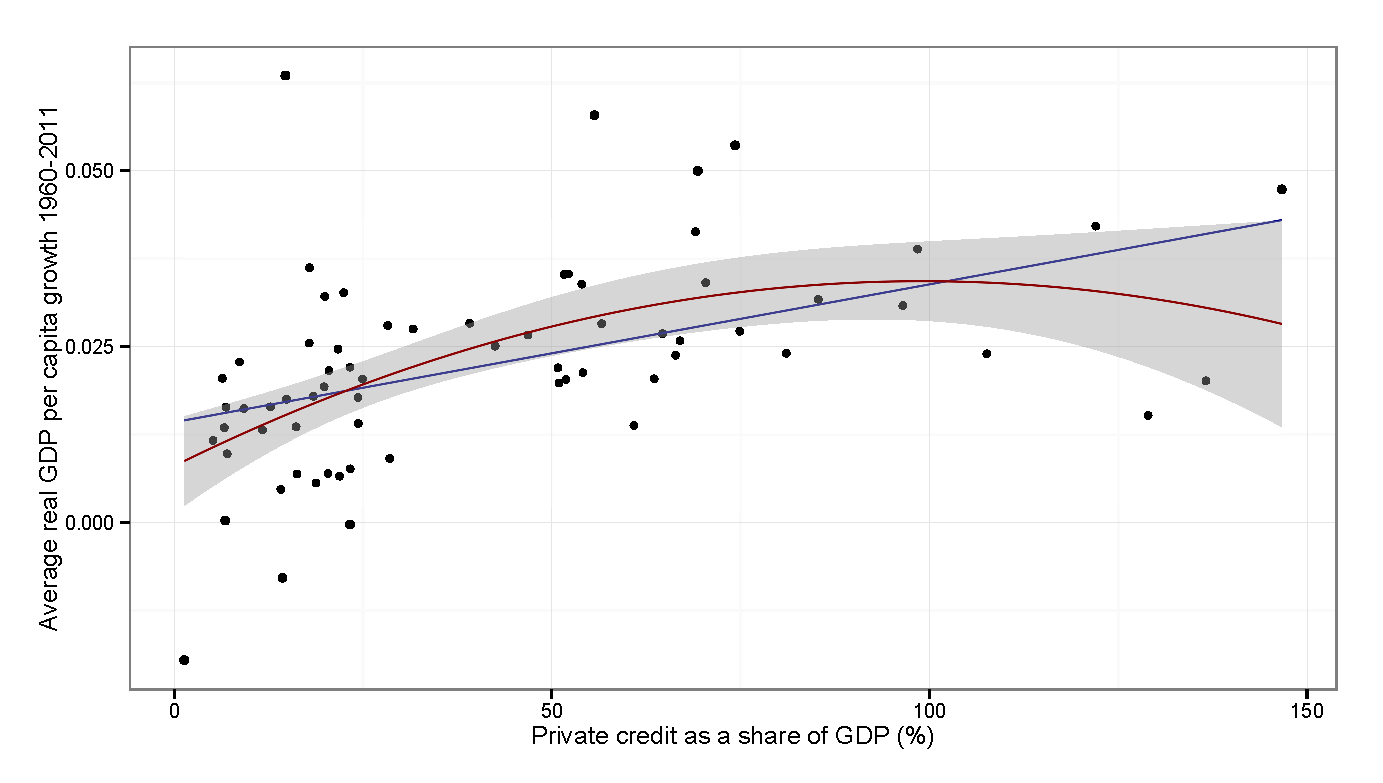
\includegraphics[width=\linewidth]{Figures/ch2/PConGDP1960-2011.eps}
\end{figure}

Table \ref{ch2tab:PC6011hyp} presents our baseline results for private credit. We sort the explanatory variables according to their \acp{PIP}. We find that the initial level of \ac{GDP} in 1960, the dummy variable for Sub-Sahara, the share of GDP in mining, the fraction of Confucian population, equipment investment, distortions in the exchange rate, and covariates capturing black market characteristics exhibit the highest \acp{PIP}. These findings are broadly in accord with the specification from \textcite{Fernandezetal2001} despite the choice of an alternative parameter prior and the consideration of an extended period. 
%
% Results, average financial indices 1960-2011; baseline results
\begin{table}[!ht]
	\centering
	\caption{Private credit and growth, baseline results\\
		Bayesian model averaging}
	\label{ch2tab:PC6011hyp}
	\footnotesize
	\begin{tabular}{lrrr}
		\toprule
		& PIP & Post Mean & Post SD \\ 
		\toprule
		Life expectancy & 1.00 & 0.00078 & 0.00023 \\ 
		GDP level in 1960 & 1.00 & -0.01330 & 0.00234 \\ 
		Fraction GDP in mining & 1.00 & 0.05972 & 0.01369 \\ 
		Fraction Confucian & 1.00 & 0.04527 & 0.01146 \\ 
		Black market premium & 1.00 & -0.01040 & 0.00327 \\ 
		Exchange rate distortions & 0.99 & -0.00009 & 0.00003 \\ 
		Sub-Sahara dummy & 0.99 & -0.01377 & 0.00539 \\ 
		SD of black market premium & 0.98 & 0.00003 & 0.00001 \\ 
		Equipment investment & 0.97 & 0.11111 & 0.04474 \\ 
		Fraction Buddhist & 0.84 & 0.00968 & 0.00653 \\ 
		Size of labor force & 0.75 & 7.1e-08 & 6.4e-08 \\ 
		French colony dummy & 0.64 & 0.00405 & 0.00402 \\ 
		Fraction Muslim & 0.53 & 0.00445 & 0.00529 \\ 
		Fraction of pop. speaking English & 0.48 & -0.00335 & 0.00445 \\ 
		Non-equipment investment & 0.38 & 0.01197 & 0.01942 \\ 
		Latin America dummy & 0.28 & -0.00152 & 0.00299 \\ 
		Rule of law & 0.24 & 0.00169 & 0.00388 \\ 
		Fraction Hindu & 0.16 & -0.00349 & 0.01138 \\ 
		Ethnolinguistic fractionalization & 0.16 & 0.00090 & 0.00268 \\ 
		Absolute latitude & 0.13 & 0.00002 & 0.00005 \\ 
		Fraction speaking foreign language & 0.11 & 0.00038 & 0.00144 \\ 
		Fraction Catholic & 0.10 & 0.00041 & 0.00180 \\ 
		British colony dummy & 0.09 & 0.00026 & 0.00133 \\ 
		Ratio of workers to population & 0.08 & 0.00059 & 0.00295 \\ 
		Public education share & 0.08 & 0.00754 & 0.03897 \\ 
		\textbf{Private credit} & \textbf{0.07} & \textbf{0.00025} & \textbf{0.00138} \\ 
		Number of years of open economy & 0.06 & -0.00030 & 0.00179 \\ 
		Spanish colony dummy & 0.06 & -0.00016 & 0.00115 \\ 
		Fraction Jewish & 0.05 & 0.00045 & 0.00319 \\ 
		Primary school enrollment & 0.05 & 0.00027 & 0.00214 \\ 
		Fraction Protestant & 0.04 & -0.00006 & 0.00108 \\ 
		Degree of capitalism & 0.04 & 0.00002 & 0.00018 \\ 
		Age & 0.03 & -5.5e-07 & 0.00001 \\ 
		Outward orientation & 0.03 & -0.00004 & 0.00043 \\ 
		High school enrollment & 0.03 & -0.00029 & 0.00572 \\ 
		Area & 0.03 & 4.9e-09 & 9.7e-08 \\ 
		Revolutions and coups & 0.03 & -0.00005 & 0.00083 \\ 
		Civil liberties & 0.03 & -0.00001 & 0.00019 \\ 
		War dummy & 0.03 & -0.00001 & 0.00036 \\ 
		Primary exports & 0.03 & -0.00001 & 0.00083 \\ 
		Population growth & 0.02 & 0.00032 & 0.02622 \\ 
		Political rights & 0.02 & -2.2e-06 & 0.00014 \\
		\bottomrule
	\end{tabular}
\end{table}
%

Although private credit ranks near the middle of the list of explanatory variables and its mean value of the coefficient is positive, the \ac{PIP} is only 7\%. This result indicates that credit is unlikely included as the explanatory variable in the ``true'' growth model. Overall, we find very limited support for the notion that financial depth is important for long-term economic growth.

In the baseline estimation, we follow \textcite{Fernandezetal2001} and use a uniform model prior. However, we depart from that study in the selection of the parameter prior. Instead of using the \ac{BRIC} prior, we employ the hyper-g prior, as the literature now considers it superior. The essential disadvantage of employing the \ac{BRIC} prior is documented by \textcite{FeldkircherZeugner2009}. They describe a phenomenon of a ``supermodel effect'', arguing that with a high fixed prior $g$, the shrinkage-factor $\frac{g}{1+g}$ in equation \ref{ch2eq:MLg} increases, thus increasing the size penalty, and may skew the posterior model distribution to smaller models. This choice of a large $g$ under fixed priors can result in a preference for overly simplistic models. According to \textcite{FeldkircherZeugner2009}, the phenomenon is characteristic of \ac{BMA} applications to growth regressions with numerous covariates. They further claim that using a model-specific hyper-g prior leads to more robust estimates. This is why we abstain from employing the \ac{BRIC} prior and focus on alternative options for parameter priors in our robustness checks.

The birth-death MC$^{3}$ sampler described in Subsection \ref{ch2sec:mc3} is our preferred approach for approximating the \ac{PMP} distribution. To ensure sufficient convergence of the sampler, we specify 15 million iterations with 3 million  initial burn-ins. The full estimation diagnostics is available upon request. The average number of regressors included in the model is 19.09, and the correlation between analytical and sampler \ac{PMP} stands at 0.56. We realize that this \ac{PMP} correlation is far from ideal, but estimation with higher iteration counts and subsequently higher \ac{PMP} correlation yields nearly identical results.\footnote{Specifically, we ran the estimation using 50 million iterations and 5 000 000 burn-ins to arrive at a \ac{PMP} correlation of 0.82. Characteristics in terms of mean model size and \acp{PIP} remain virtually the same.} Note that below, we employ different parameters and model prior structures and achieve a \ac{PMP} close to 1, while the \acp{PIP} remain largely unchanged. 

Next, we examine whether the baseline results are robust to different parameter priors. \textcite{CicconeJarocinski2010} posit that \ac{BMA} results are sensitive to data revisions under certain prior structures. \textcite{Eicheretal2011} find that the \acp{PIP} of some growth determinants depend on the chosen parameter prior. Therefore, we perform the estimation using \ac{UIP}. We also check the robustness of the MC$^{3}$ sampler using the ``reverse-jump'' algorithm and the model prior by employing a random binomial model prior (see \textcite{Zeugner2011} for details).

The model comparison for different parameter priors and MC$^{3}$ algorithms is depicted in Figure \ref{ch2fig:compPC}. Model 1 includes the \acp{PIP} under our baseline specification. Model 2 employs the same priors but applies the ``reverse-jump'' MC$^{3}$ algorithm. Models 3 and 4 yield the results when we use \ac{UIP} under the birth-death and reverse-jump samplers, respectively. Though employing the reverse-jump sampler only marginally alters the \acp{PIP}, switching to the \ac{UIP} prior leads to slightly lower inclusion probabilities and model size. Overall, these findings indicate that our baseline results are robust.

% 
% Model comparison, 1960-2011 PC
\begin{figure}[!ht]
		\centering
		\caption{Model comparison with private credit}
		\label{ch2fig:compPC}
		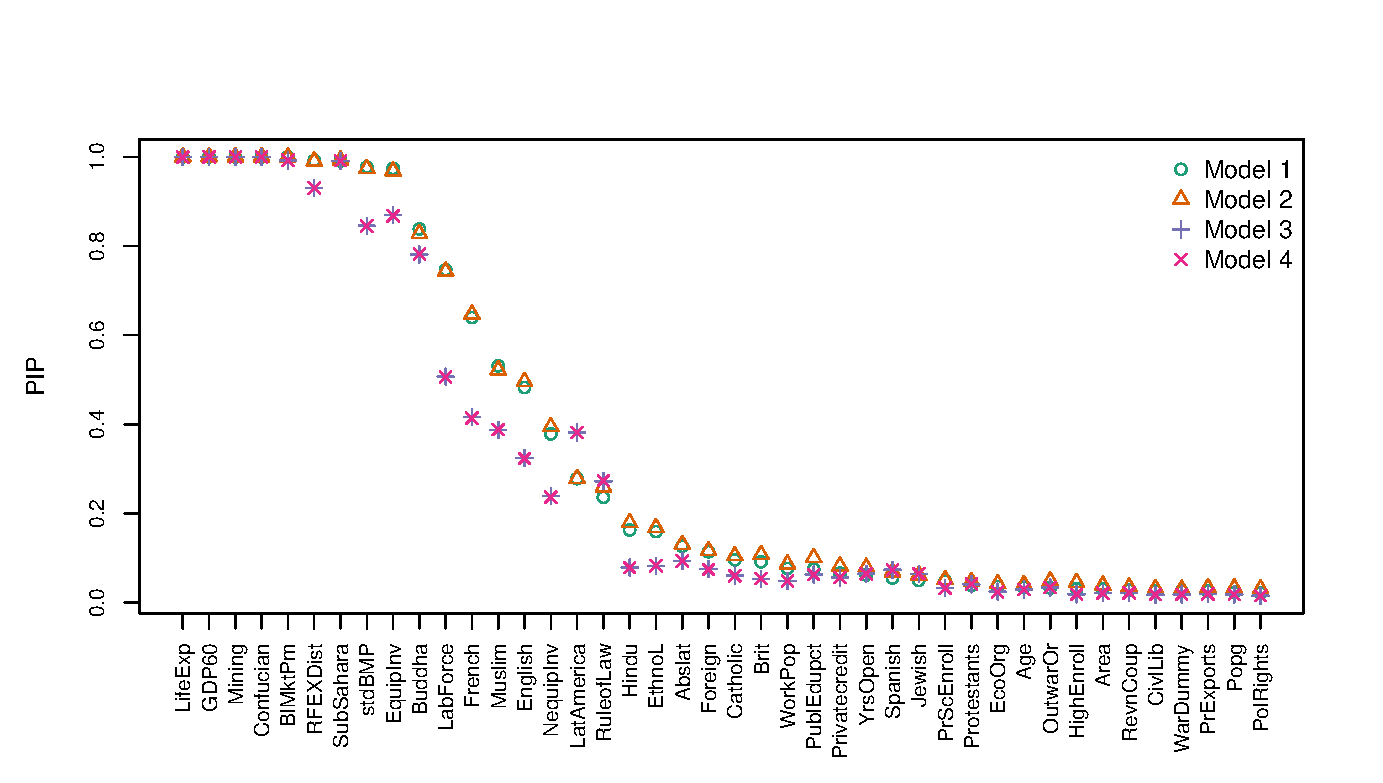
\includegraphics[width=\linewidth]{Figures/ch2/plotCompPC6011}
	 \begin{minipage}{0.8\textwidth}
		\footnotesize
		\emph{Note: Model 1=hyper-g,birth-death; Model 2=hyper-g,reverse-jump; Model 3=\ac{UIP},birth-death; Model 4=\ac{UIP},reverse-jump}
	  \end{minipage}
\end{figure}
%

The beta-binomial (``random'') model prior offers meaningful insights. This setting allows for a less restrictive selection of model priors around the prior expected model size and limits the risk of imposing any particular one \parencite{LeySteel2009}. Thus, if the true model size is lower than that expected by the prior (21), we should expect the mean model size to decline in this setting. 
%
We present the results of the estimation using this model prior in Figure \ref{ch2fig:compPCrnd} in the Appendix. In the first setting with a hyper-g prior, the mean size declines to 15.05 and the PMP correlation between analytical and MC$^{3}$ sampler likelihood achieves a satisfactory value of 0.96. The most important variables according to their \acp{PIP} remain nearly unchanged, although their relative positions adjust. One significant change is the decline in the PIP of the volatility of the black market premium to 14\%. Finally, the inclusion probability of private credit increases marginally to 9\%. 

We also limit the period under consideration to 1960-1990 and examine whether the effect of financial development is stronger for this time period, as suggested by \textcite{RousseauWachtel2011}. We find that none of these modifications substantially affects our primary results concerning the relationship between private credit and economic growth.  The PIP of private credit estimated on the subsample before 1990 does not appear to differ from that obtained for the full period up to 2011. As a robustness check of our results, we also use the values of private credit from the beginning of the observed period instead of the averages, but we find that the coding change has a negligible effect. These results are available upon request.

\subsection{New Financial Development Indicators}
We examine the effect of new financial indicators on long-term growth in this subsection. Specifically, we additionally include the following variables in our estimation: bank Z-score, net interest margin, stock market turnover, and stock market capitalization. \textcite{Cihaketal2013} identify these as proxies for different aspects of the financial sector. Specifically, they propose using bank Z-score to assess the stability of the banking sector, the net interest margin to proxy for the efficiency of the banking sector, stock market turnover as a proxy for the efficiency of the stock market, and stock market capitalization to measure the depth of stock markets. These measures, particularly the first two, are rarely used in growth regressions (\textcite{Bergeretal2004} and \textcite{Hasanetal2009} being the exceptions), despite the fact that they might better depict the relationships outlined by theory than traditionally employed variables. As we discuss in Section \ref{ch2sec:data}, the main issue lies in their availability. However, the \ac{GFDD} provides a significant improvement in this regard, and many series are available since the late 1980s. In addition, we retain domestic credit to the private sector among the covariates to account for the overall size of the banking sector. Given the data limitations, our sample is reduced to 60 countries. For eight countries from our original sample used for private credit, at least one value of the new financial indicators is missing.

Figure \ref{ch2fig:allvarplot} provides an initial examination of the interaction between individual financial indicators and economic growth. First, we observe a distinct inverse relationship between the net interest margin and economic growth. Second, bank Z-score and growth display only a marginally positive relationship. Third, market capitalization and market turnover appear to be positively related to growth, which is in line with \textcite{LevineZervos1998}. In addition, Table \ref{ch2tab:corrFI} provides the correlations among the financial indicators. The correlations are typically far from one, thus providing additional impetus to examine further measures of financial development in the growth regressions. In addition, we present the jointness statistics in the Appendix \ref{ch2app:joint}.
%
% Rest of the financial indicators 1960-2011
\begin{figure}[!ht]
	\centering
	\caption{Financial indicators and growth}
		\label{ch2fig:allvarplot}
		% \setlength{\fboxsep}{0pt}
		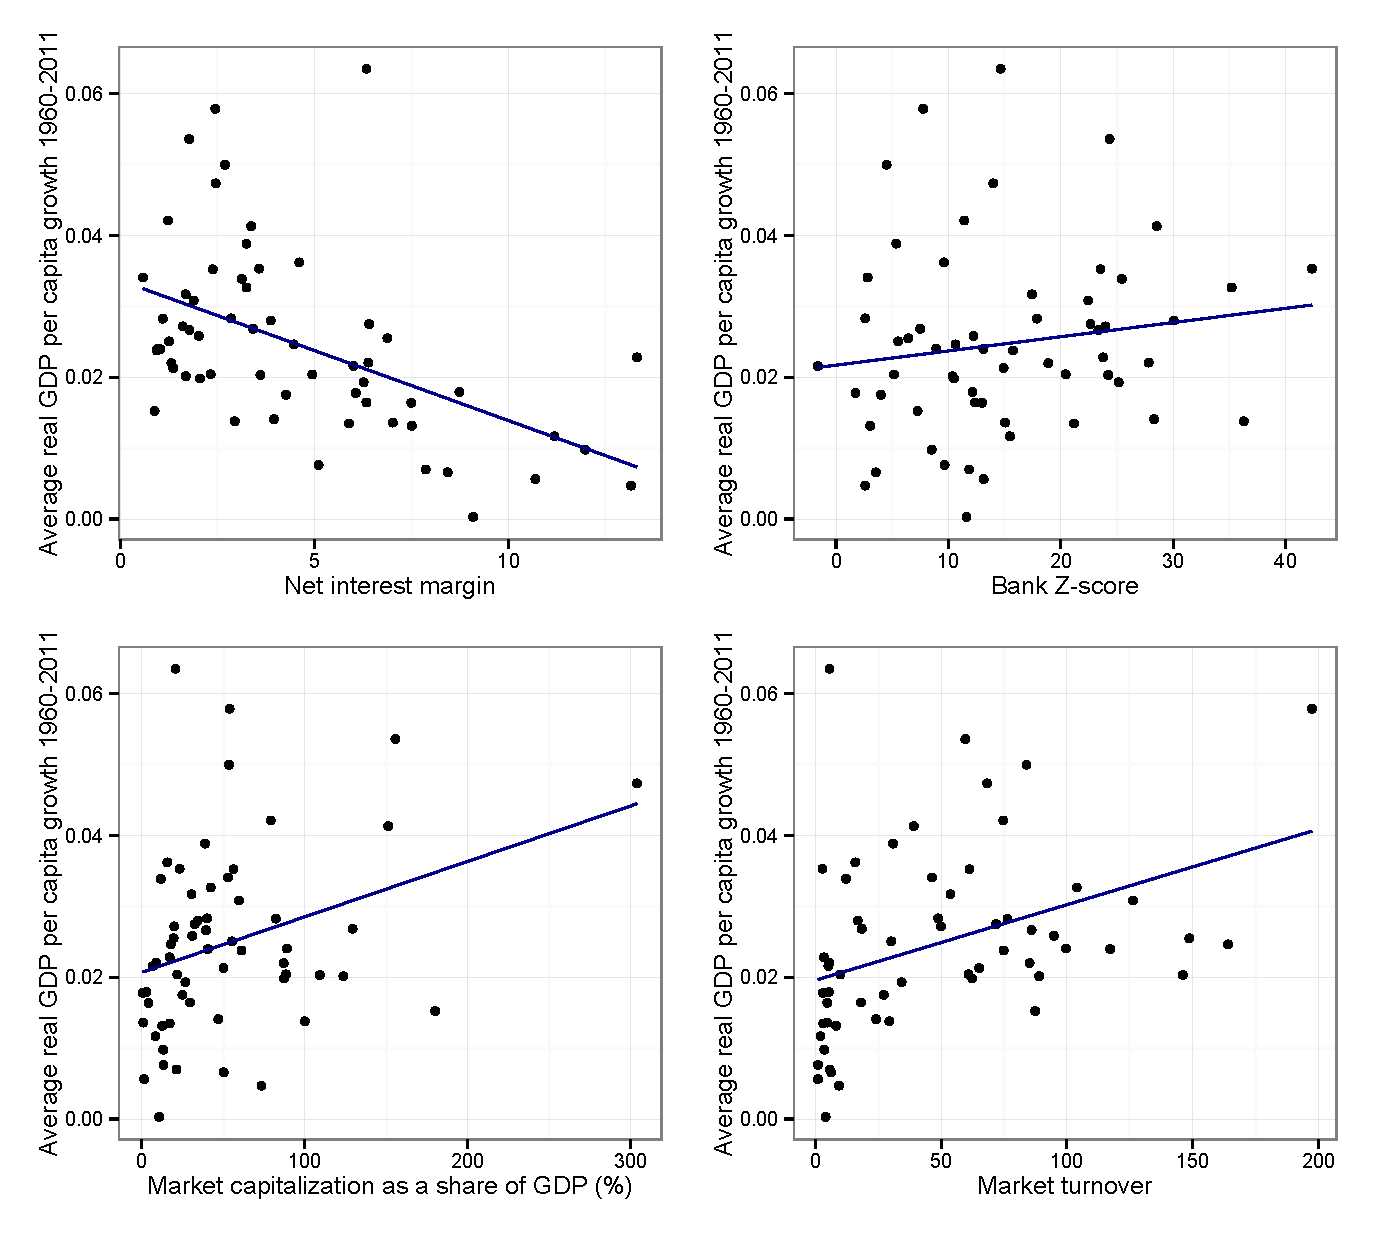
\includegraphics[width=\linewidth]{Figures/ch2/Plots60}
\end{figure}
%
% Correlation matrix of financial indicators
\begin{table}[!ht]
	\centering
	\caption{Correlation matrix of new financial indicators}
	\label{ch2tab:corrFI}
	\small
	\begin{tabular}{lrrrrr}
		\toprule
		Net interest margin & 1.00 & & & &                    \\ 
		Bank Z-score    & -0.14 & 1.00 &   &   &              \\ 
		Private credit & -0.71 & 0.03 & 1.00 &   &            \\ 
		Market capitalization & -0.44 & 0.08 & 0.71 & 1.00 &  \\ 
		Market turnover & -0.54 & 0.02 & 0.47 & 0.33 & 1.00   \\ 
		\bottomrule
	\end{tabular}
\end{table}
%

We report the results of the estimation in a similar fashion as we did for private credit. We retain the baseline specification with the hyper-g parameter prior, uniform model prior, and birth-death MC$^{3}$ sampler. The number of iterations remains at 15 million, and we specify 3 million burn-ins. The full estimation diagnostics is available upon request. As in the previous subsection, running more iterations does not affect the resulting \acp{PIP} and posterior means, although it leads to a higher convergence of the sampler. We primarily focus on the interpretation of the results concerning financial indicators, as the other explanatory variables' \acp{PIP} remain broadly similar to those of specification for private credit. 

%\clearpage
% All financial indicators, baseline results
\begin{table}[!htbp]
	\centering
	\caption{New financial indicators and growth 1960-2011, baseline results}
	\label{ch2tab:all6011hyp}
	\footnotesize
	\begin{tabular}{lrrr}
		\toprule
		& PIP & Post Mean & Post SD \\ 
		\midrule
		GDP level in 1960 & 1.00 & -0.01075 & 0.00234 \\ 
		Fraction GDP in mining & 1.00 & 0.04669 & 0.01338 \\ 
		Exchange rate distortions & 1.00 & -0.00009 & 0.00003 \\ 
		Fraction Confucian & 1.00 & 0.03896 & 0.01093 \\ 
		Life expectancy & 1.00 & 0.00057 & 0.00019 \\ 
		Fraction Buddhist & 0.98 & 0.01255 & 0.00497 \\ 
		\textbf{Net interest margin} & \textbf{0.97} & \textbf{-0.00115} & \textbf{0.00045} \\ 
		Equipment investment & 0.85 & 0.07432 & 0.04648 \\ 
		\midrule
		Fraction Protestant & 0.33 & -0.00225 & 0.00402 \\ 
		Ratio of workers to population & 0.33 & 0.00382 & 0.00671 \\ 
		\textbf{Bank Z-score} & \textbf{0.25} & \textbf{0.00004} & \textbf{0.00009} \\ 
		French colony dummy & 0.24 & 0.00183 & 0.00411 \\ 
		SD of black market premium & 0.22 & 3.1e-06 & 0.00001 \\ 
		Rule of law & 0.19 & 0.00139 & 0.00363 \\ 
		Outward orientation & 0.19 & -0.00050 & 0.00133 \\ 
		\textbf{Market turnover} & \textbf{0.17} & \textbf{0.00001} & \textbf{0.00002} \\ 
		Size of labor force & 0.12 & 6.6e-09 & 2.6e-08 \\ 
		Spanish colony dummy & 0.12 & 0.00054 & 0.00192 \\ 
		Fraction of pop. speaking English & 0.11 & -0.00044 & 0.00168 \\ 
		Fraction Jewish & 0.08 & 0.00093 & 0.00423 \\ 
		Fraction Muslim & 0.08 & 0.00033 & 0.00158 \\ 
		\textbf{Private credit} & \textbf{0.07} & \textbf{0.00028} & \textbf{0.00145} \\ 
		Fraction Catholic & 0.07 & -0.00025 & 0.00139 \\ 
		Primary exports & 0.06 & 0.00020 & 0.00135 \\ 
		Absolute latitude & 0.05 & 4.2e-06 & 0.00003 \\ 
		Fraction Hindu & 0.05 & -0.00048 & 0.00435 \\ 
		Fraction speaking foreign language & 0.05 & 0.00009 & 0.00068 \\ 
		Population growth & 0.04 & -0.00554 & 0.04705 \\ 
		Number of years of open economy & 0.04 & 0.00011 & 0.00093 \\ 
		Age & 0.04 & -6.6e-07 & 0.00001 \\ 
		War dummy & 0.04 & -0.00005 & 0.00047 \\ 
		High school enrollment & 0.04 & -0.00061 & 0.00575 \\ 
		Latin America dummy & 0.04 & -0.00006 & 0.00079 \\ 
		Black market premium & 0.04 & 0.00010 & 0.00101 \\ 
		Non-equipment investment & 0.04 & -0.00040 & 0.00408 \\ 
		Political rights & 0.04 & 0.00002 & 0.00018 \\ 
		British colony dummy & 0.04 & -0.00001 & 0.00045 \\ 
		Area & 0.03 & 7.9e-09 & 8.9e-08 \\ 
		Degree of capitalism & 0.03 & 0.00002 & 0.00019 \\ 
		Public education share & 0.03 & 0.00078 & 0.01915 \\ 
		Revolutions and coups & 0.03 & -0.00005 & 0.00076 \\ 
		Sub-Sahara dummy & 0.03 & -0.00001 & 0.00087 \\ 
		Primary school enrollment & 0.03 & -0.00007 & 0.00129 \\ 
		Ethnolinguistic fractionalization & 0.03 & -0.00001 & 0.00064 \\ 
		\textbf{Market capitalization} & \textbf{0.02} & \textbf{1.1e-07} & \textbf{3.3e-06} \\
		Civil liberties & 0.02 & 0.00001 & 0.00016 \\ 
		\bottomrule 
	\end{tabular}
\end{table}

We present the posterior statistics of the explanatory variables in Table \ref{ch2tab:all6011hyp}. Interestingly, the variable proxying for bank efficiency exhibits a comparatively higher \ac{PIP} than that reflecting its depth. Net interest margin ranks high among the explanatory variables with a 97\% inclusion probability. The posterior mean of the coefficient is negative, in accordance with our expectations. A lower interest margin stems from a smaller discrepancy between banks' borrowing and lending rates. Thus, if banks are able to channel resources at a lower margin, this appears to positively affect long-term economic growth \parencite{Rousseau1998}. Additionally, the posterior mean of bank Z-score is positive, implying that stable banking systems are beneficial for economic growth, although the \ac{PIP} at 25\% does not offer much confidence that the Z-score is a crucial determinant of long-term growth. Stock market turnover is also accorded little importance, with a \ac{PIP} of 17\%. The positive sign of the mean is in line with our expectations regarding an efficient resource allocation being beneficial for growth. Moreover, it supports the conclusion of \textcite{LevineZervos1998} that an active stock market contributes to economic growth. However, we wish to note that this indicator might not coherently capture the efficiency of the markets. A high turnover ratio could reflect low friction in trading and the spread of information \parencite{Levine2005}. On the other hand, other research finds that more trading does not necessarily prevent asset price misalignments and its corrections \parencite{Brunnermeier2004}. Strikingly, the measures capturing the depth of both the banking sector and stock markets exhibit very small \acp{PIP}. Overall, our results indicate that the approach used to measure financial development is crucial in determining the estimated effect of finance on growth. 

To provide robustness checks, we again perform the estimation with alternative priors.\footnote{We also perform estimations using an alternative MC$^{3}$ sampler, but the differences in posterior statistics are marginal.} Figure \ref{ch2fig:compall60} illustrates the comparison. The implications of different priors are similar to those experienced in the estimation regarding private credit. The \ac{UIP} parameter prior subtly alters the \ac{PIP} of the covariates without having a major effect on the interpretation. Providing greater flexibility in selecting model size by assuming a random model prior reduces the posterior mean model size and the \ac{PIP} of several variables, but the set of top-ranked regressors remains largely unchanged. The relative importance of financial indicators changes to some extent. Net interest margin remains among the most important variables with an 86\% \ac{PIP}. All the remaining indicators exhibit low \ac{PIP} below 10\%. This is due to the smaller size induced by the random model prior. The results using dilution prior which accounts for correlation among covariates decreases the \ac{PIP} of nearly all variables. However, the importance of net interest margin still remains high with the \ac{PIP} at 87\%.
% Model comparison, 1960-2011 findev
\begin{figure}[!ht]
	\centering
	\caption{Model comparison with all financial indicators 1960-2011}
		\label{ch2fig:compall60}
		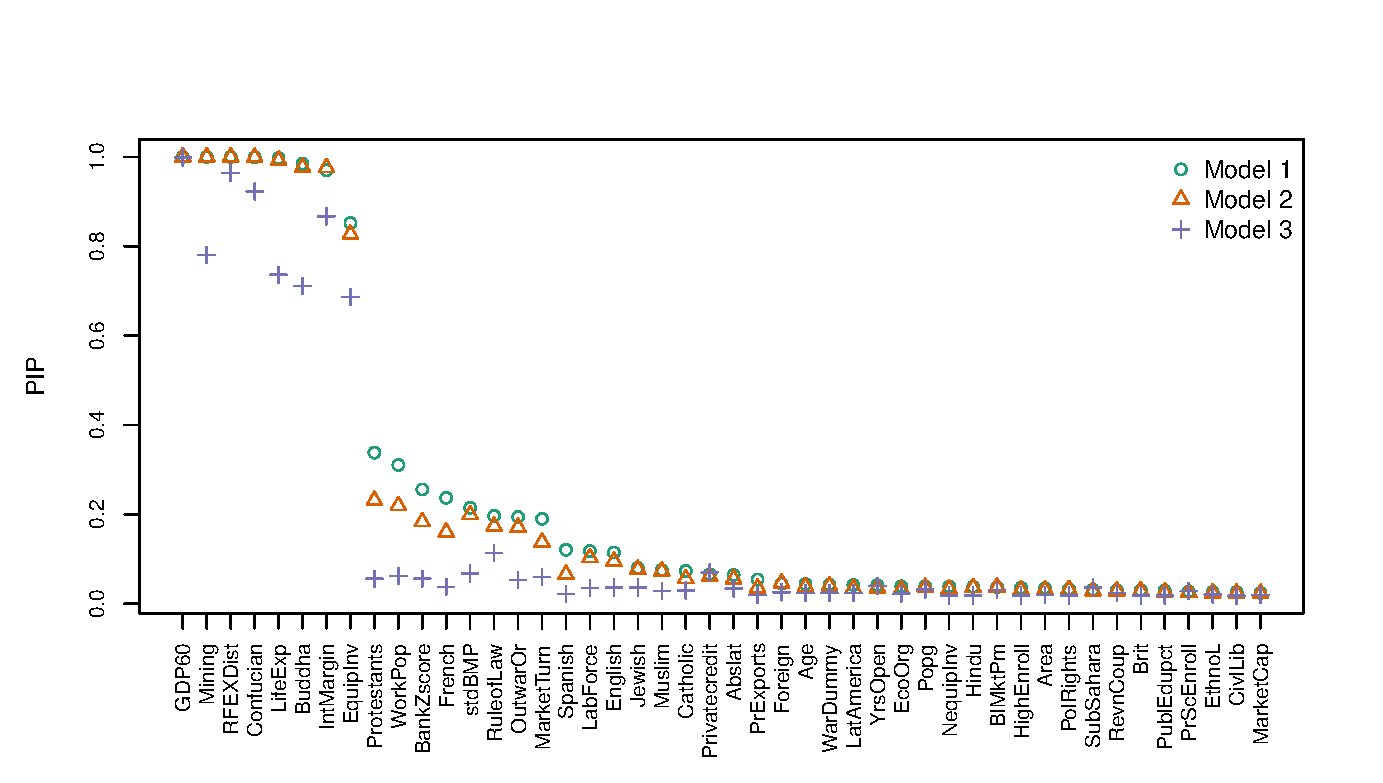
\includegraphics[width=\linewidth]{Figures/ch2/plotCompall6011}
		\begin{minipage}{0.8\textwidth}
			\footnotesize
			\emph{Note: Parameter and model prior comparison. Model 1=hyper-g, uniform model prior; Model 2=\ac{UIP}, uniform model prior, Model 3=hyper-g, dilution model prior}
		  \end{minipage}
\end{figure}

\subsection{Addressing endogeneity}\label{ch2subsec:endog}
Our dataset is constructed such that most regressors are exogenous except for certain financial indicators. While we efficiently tackle the potential for omitted variable bias by allowing for many potential regressors by using \ac{BMA}, the issue of reverse causality of the relationship remains a challenge. In particular, the class of endogenous growth models points towards the reciprocal relation between growth and financial development. In these models, the demand for financial services grows with an increased level of economic development. The higher demand for financial services boosts competition and improves the efficiency of financial intermediation. Simultaneously, the finance's better efficiency enhances the screening and capital allocation of investment, accelerating capital accumulation, and consequently, economic growth \parencite{Ang2008}. In the short run, economic development affects financial sector and some of the indicators we use to proxy for financial development. Credit provision traditionally decreases in recessions, so does the stock market capitalization. Apart from interdependence between economic growth and finance put forward in theory, some empirical studies thus document the dynamics between financial crises  \parencite{cerra2008growth,DellAricciaetal2008} or financial liberalization \parencite{Ranciereetal2006} and parallel changes of output. By focusing on the long-run relationship, we abstract from these dynamics.

To address the potential endogeneity of financial indicators, we apply the methodology developed by \textcite{Durlaufetal2008}. The endogenous financial variables are regressed on a set of instruments in the first stage, and their fitted values are used in the second stage, which is a standard BMA procedure. We acknowledge that the first stage is not fully Bayesian, but it is important to note that the number of endogenous variables and instruments is rather low. In addition, \textcite{Durlaufetal2008} performs Monte Carlo simulations and shows that this two-stage least squares BMA approach (2SLS-BMA) approximates the data generating process accurately. In the estimations, we build on the baseline results and address mainly the potential endogeneity of the net interest margin. 

We use the data from \textcite{ReinhartRogoff2008} on the history of financial crises as the instruments. We have tried different alternatives as instruments, such as the data on financial reform compiled by \textcite{Abiadetal2008}. This choice is popular in the literature, but we found that the data on financial crises have much better explanatory power.

% The financial reform index incorporates information on credit conditions, financial market supervision, and competition characteristics. It represents the reform inputs (which are typically initiated by international organizations such as the International Monetary Fund) and not reform outcomes; therefore, it is likely to be independent of growth. Moreover, previous research shows that financial reforms spur financial development \parencite{JayaratneStrahan1996,TresselDetragiache2008}. In addition, the key characteristic of financial development is its continuity, and financial reform reversals may have particularly devastating effects on financial development \parencite{RajanZingales2003}. Therefore, using the data in \textcite{Abiadetal2008}, we include the average size of the reversal of financial reform (the reversal is defined as the decrease in the index value, and the average value of reversals is used as the instrument) and the total number of large reversals over the observed period (we consider a large reversal to be a decrease in the non-standardized index value larger than 3). 

\textcite{ReinhartRogoff2008} recognize several types of financial distress: currency, inflation, debt, bank crises and stock market crashes. Furthermore, they distinguish between domestic and external debt crises. For each year, they assign a value of 1 if a particular type of crisis occurs. The total crisis tally in a year can therefore take values from 0 to 6. We believe that the legacy of troubled financial systems may be deeply rooted in the economy and have a long-term impact on financial development. For example, \textcite{Guiso2008} show how a lack of trust leads to lower stock market participation. Specifically, we consider the average crisis tally (average number of crises per year) in the countries over the period of their independence. The relationship between financial crises and economic growth is likely to be only temporary, with the effect eventually diminishing \parencite{Ranciereetal2006}. Therefore, their occurrence is likely unrelated to long-term growth\footnote{Additionally, we also estimate the 2SLS--BMA with the crises values only considering the data before 1960 to strengthen the exogeneity argument. The \ac{PIP} of the net interest margin decreases slightly to 0.8, but generally the results remain the same.}. To the instrument, which ensures the identification of the two-stage model, we add the rule of law and the years for which the country has had an open economy as additional regressors. \textcite{RajanZingales2003} and \textcite{Baltagietal2009} identify these two variables as determinants of financial development. In addition, these two variables exhibit high correlation with most of our financial indicators. Furthermore, absolute latitude is included to control for the geographical endowment of individual countries. Latitude is exogenous to growth and is shown to correlate with financial development \parencite{Becketal2002, Becketal2003}. 

Crises data are not available for all countries. To prevent reducing our sample, in exceptional cases, we use the regional averages for missing data. The regions are defined as follows: Sub-Saharan Africa, Latin America and the rest of the world\footnote{The countries for which we are missing data are Botswana, Cyprus, Hong Kong, Israel, Jamaica, Jordan, Malawi, Pakistan, Tanzania, Uganda.}.

Table \ref{ch2tab:all6011hypIValt} reports the results using 2SLS-BMA estimation. The results from the first-stage regression is presented in the appendix in Table \ref{app1tab:1ststageIV}. Among the top regressors, there are no apparent qualitative differences between the baseline and 2SLS-BMA results. The posterior inclusion probability of net interest margin remains high at 92\%. The PIP for bank Z-score and market capitalization decline to very low levels. Private credit and stock market capitalization, the traditional financial development proxies, continue to display low inclusion probabilities.

\begin{table}[!htbp]
	\centering
	\caption{New financial indicators and growth 1960-2011, \\ 2SLS--BMA}
	\label{ch2tab:all6011hypIValt}
	\small
	\begin{tabular}{lrrr}
	 	  \toprule
		  & PIP & Post Mean & Post SD \\ 
		  \midrule
		  GDP level in 1960 & 1.00 & -0.01171 & 0.00252 \\
  Fraction GDP in mining & 1.00 & 0.04670 & 0.01290 \\ 
  Exchange rate distortions & 1.00 & -0.00009 & 0.00003 \\
  Life expectancy & 1.00 & 0.00059 & 0.00020 \\ 
  Fraction Confucian & 0.99 & 0.04077 & 0.01183 \\ 
  Fraction Buddhist & 0.94 & 0.01143 & 0.00558 \\
  \textbf{Net interest margin} & \textbf{0.92} & \textbf{-0.00148} & \textbf{0.00072} \\
  Equipment investment & 0.87 & 0.08065 & 0.04660 \\
  Fraction Protestants & 0.62 & -0.00482 & 0.00505 \\ 
  Size of labour force & 0.39 & 0.00000 & 0.00000 \\
  Outward orientation & 0.38 & -0.00121 & 0.00191 \\
  Ratio of workers to population & 0.28 & 0.00303 & 0.00596 \\ 
  Fraction Jewish & 0.26 & 0.00381 & 0.00821 \\ 
  Fraction of pop. speaking English & 0.24 & -0.00128 & 0.00287 \\ 
  Bank Z-score & 0.22 & 0.00004 & 0.00009 \\ 
  Rule of law & 0.20 & 0.00175 & 0.00432 \\ 
  Primary exports & 0.19 & 0.00143 & 0.00377 \\
  Market turnover & 0.18 & 0.00001 & 0.00002 \\ 
  Fraction Hindu & 0.18 & -0.00455 & 0.01298 \\ 
  SD of black market premium & 0.15 & 0.00000 & 0.00001 \\ 
  French colony dummy & 0.15 & 0.00101 & 0.00319 \\ 
  Private credit & 0.13 & 0.00001 & 0.00002 \\ 
  Fraction speaking foreign language & 0.11 & 0.00031 & 0.00127 \\ 
  Spanish colony dummy & 0.11 & 0.00052 & 0.00200 \\ 
  Political rights & 0.10 & 0.00010 & 0.00042 \\ 
  Fraction Catholic & 0.10 & -0.00035 & 0.00160 \\ 
  Population growth & 0.09 & -0.02058 & 0.08788 \\ 
  High school enrolment & 0.08 & -0.00210 & 0.01155 \\ 
  Age & 0.07 & -0.00000 & 0.00001 \\ 
  Public education share & 0.06 & 0.00493 & 0.03187 \\ 
  Sub-Sahara dummy & 0.06 & 0.00006 & 0.00153 \\
  Civil liberties & 0.06 & 0.00003 & 0.00032 \\
  Fraction Muslim & 0.05 & 0.00007 & 0.00142 \\
  Absolute latitude & 0.05 & 0.00000 & 0.00003 \\
  Latin America dummy & 0.05 & -0.00012 & 0.00115 \\
  Degree of capitalism & 0.05 & 0.00003 & 0.00023 \\ 
  Number of years of open economy & 0.04 & 0.00010 & 0.00107 \\ 
  Market capitalization & 0.04 & 0.00000 & 0.00000 \\
  British colony dummy & 0.04 & -0.00004 & 0.00051 \\
  War dummy & 0.03 & 0.00001 & 0.00037 \\ 
  Area & 0.03 & 0.00000 & 0.00000 \\ 
  Black market premium & 0.03 & 0.00007 & 0.00087 \\
  Revolutions and coups & 0.03 & -0.00001 & 0.00073 \\ 
  Ethnolinguistic fractionalization & 0.03 & 0.00002 & 0.00068 \\
  Primary school enrolment & 0.03 & -0.00005 & 0.00134 \\
  Non-equipment investment & 0.02 & 0.00006 & 0.00284 \\  
  	 \bottomrule
	\end{tabular}
\end{table}

Our baseline and 2SLS--BMA estimations suggest that bank efficiency is crucial for growth. We perform an additional estimation to check the robustness of this finding and estimate \ac{BMA} with lagged covariates. For reasons of data availability, we use real growth in GDP per capita over the period 2000--2011 and take the values of the financial indicators in the year 2000. The advantage of this approach is that we examine how past values of financial indicators influence current growth. Clearly, the disadvantage is that the time coverage for the dependent variable is restricted to just over a decade. Implicitly, this may also be regarded as robustness check of the sensitivity of our results to the variable coding. We present the results in Table \ref{ch2tab:BMAgrowth2000-2011}. Interestingly, the results remain largely unchanged. Net interest margin remains among the covariates with the highest \ac{PIP}. The posterior mean of the coefficient is negative. The \ac{PIP} of private credit is 49\%, but the mean is negative. We hypothesize that the negative mean is a consequence of our sample period including the current global financial crisis, which has been characterized by deleveraging in many developed countries. The \ac{PIP} of the other financial indicators is low.

We alternate between different approaches towards endogeneity as each of them has its limits. The use of lagged variables and limiting the sample for a relatively short and specific period of the 2000s may not well capture the relationship's long-run nature and may be affected by the business cycle dynamics. On the other hand, the instrumental variable approach relies heavily on good instrument choice, and their qualification may almost universally be disputed\footnote{See \textcite{deaton2010instruments} for a critical overview of the use of instruments in economics and further references}. The choice of weak instruments may also generate more biased estimates than the elementary approaches, such as OLS \parencite{bazzi2013blunt}. The alternative estimation strategies we employ provide additional evidence for our baseline results and support the finance-led hypothesis.

\begin{table}[!htbp]
	\centering
	\caption{New financial indicators and growth 2000-2011, baseline results}
		\label{ch2tab:BMAgrowth2000-2011}
	\footnotesize
	\begin{tabular}{lrrr}
		\toprule
		& PIP & Post Mean & Post SD \\ 
		\midrule
		  Exchange rate distortions & 1.00 & 0.00022 & 0.00004 \\ 
		  War dummy & 1.00 & 0.01149 & 0.00290 \\ 
		  \textbf{Net interest margin} & \textbf{1.00} & \textbf{-0.00212} & \textbf{0.00055} \\ 
		  Primary exports & 1.00 & 0.01699 & 0.00496 \\ 
		  Fraction Confucian & 1.00 & 0.04151 & 0.01130 \\ 
		  Non-equipment investment & 1.00 & -0.09469 & 0.02661 \\ 
		  Political rights & 1.00 & 0.00641 & 0.00152 \\ 
		  Latin America dummy & 1.00 & 0.01679 & 0.00470 \\ 
		  Fraction GDP in mining & 1.00 & 0.08843 & 0.01789 \\ 
		  Ratio of workers to population & 1.00 & 0.04116 & 0.00919 \\ 
		  Revolutions and coups & 1.00 & -0.03279 & 0.00649 \\ 
		  Outward orientation & 1.00 & 0.00900 & 0.00261 \\ 
		  Sub-Sahara dummy & 1.00 & -0.03589 & 0.00910 \\ 
		  Fraction Hindu & 0.94 & 0.03725 & 0.01387 \\ 
		  SD of black market premium & 0.88 & 0.00003 & 0.00002 \\ 
		  \textbf{Private credit} & \textbf{0.53} & \textbf{-0.00003} & \textbf{0.00004} \\ 
		  Life expectancy & 0.31 & 0.00011 & 0.00021 \\ 
		  High school enrolment & 0.25 & -0.00932 & 0.02257 \\ 
		  \textbf{Bank Z-score} & \textbf{0.21} & \textbf{-0.00004} & \textbf{0.00010} \\ 
		  Rule of law & 0.16 & 0.00106 & 0.00369 \\ 
		  French colony dummy & 0.15 & -0.00091 & 0.00311 \\ 
		  Degree of capitalism & 0.14 & 0.00014 & 0.00055 \\ 
		  Size of labour force & 0.13 & 1.3e-08 & 5.0e-08 \\ 
		  Black market premium & 0.12 & 0.00084 & 0.00375 \\ 
		  Spanish colony dummy & 0.11 & -0.00046 & 0.00250 \\ 
		  Civil liberties & 0.10 & -0.00018 & 0.00096 \\ 
		  Number of years of open economy & 0.09 & 0.00034 & 0.00206 \\ 
		  Age & 0.09 & 1.1e-06 & 0.00001 \\ 
		  GDP level in 2000 & 0.09 & 0.00009 & 0.00076 \\ 
		  British colony dummy & 0.08 & 0.00004 & 0.00079 \\ 
		  Public education share & 0.08 & 0.00470 & 0.03815 \\ 
		  Absolute latitude & 0.08 & 4.3e-06 & 0.00003 \\ 
		  Fraction Muslim & 0.08 & 0.00035 & 0.00215 \\ 
		  Population growth & 0.08 & -0.00603 & 0.07020 \\ 
		  \textbf{Market capitalization} & \textbf{0.07} & \textbf{3.8e-07} & \textbf{4.7e-06} \\ 
		  Fraction Buddhist & 0.07 & -0.00021 & 0.00167 \\ 
		  Fraction Catholic & 0.07 & -0.00012 & 0.00102 \\ 
		  Ethnolinguistic fractionalization & 0.07 & 0.00028 & 0.00171 \\ 
		  Primary school enrolment & 0.07 & 0.00026 & 0.00278 \\ 
		  \textbf{Market turnover} & \textbf{0.07} & \textbf{4.5e-07} & \textbf{3.7e-06} \\ 
		  Fraction Jewish & 0.07 & 0.00017 & 0.00230 \\ 
		  Area & 0.07 & 1.3e-08 & 1.3e-07 \\ 
		  Fraction speaking foreign language & 0.07 & 0.00011 & 0.00089 \\ 
		  Fraction Protestants & 0.06 & 0.00007 & 0.00107 \\ 
		  Fraction of pop. speaking English & 0.05 & -0.00011 & 0.00103 \\ 
		  Equipment investment & 0.04 & 0.00026 & 0.00815 \\ 
		\bottomrule
	\end{tabular}
\end{table}

\subsection{Non--linearities in Finance and Growth Nexus}\label{ch2subsec:nonlin}
Finally, we examine the possibility of a nonlinear relationship between financial indicators and growth. Several recent studies on financial development and economic growth devote substantial attention to nonlinearities in the relationship between financial development and economic growth (see, for example, \textcite{CecchettiKharroubi2012, LawSingh2014}). In addition, we also examine several possible interaction effects in finance--growth nexus such as whether private credit is conducive to growth only when financial system is stable.

When considering the quadratic and interaction terms, we rely on the strong heredity principle to adjust prior model probabilities. This approach has been suggested in the literature to ensure appropriate interpretation of the results. In essence, the quadratic and interaction terms may only be evaluated when their linear counterparts are included in the model. Therefore, they cannot mask potential effects of linear terms. 

The results of the specification focused only on private credit do not alter our conclusions from the basic linear setup. The posterior inclusion probabilities of private credit and its quadratic term are 8\% and 1\%, respectively.\footnote{In this subsection we report only the posterior statistics of the financial variables. The full results including the other variables are available upon request.} Next, we present the results with all financial indicators in Table \ref{ch2fig:BMAquad}. The \acp{PIP} on the linear terms are similar to the ones in the baseline linear specification from the previous subsection. The \ac{PIP} on the net interest margin remains high at 88\%. At the same time, we find very low posterior inclusion probabilities for all the quadratic terms with the exception of the net interest margin, which stands at 38\%. While this value is not higher than sometimes suggested cut-off threshold of 50\%, it provides some weak evidence for decreasing marginal returns of our efficiency indicator. 

\begin{table}[!htbp]
	\centering
	\caption{New financial indicators and quadratic terms\\
		Bayesian model averaging}
		\label{ch2fig:BMAquad}
	\small
	\begin{tabular}{lrrr}
		\toprule
		& PIP & Post Mean & Post SD \\ 
		\midrule
		  Net interest margin & 0.88 & -0.00192 & 0.00155\\ 
		  Net interest margin sq. & 0.38 & 0.00006 & 0.00010\\ 
		  Market turnover & 0.20 & 0.00003 & 0.00009\\ 
		  Bank Z-score & 0.19 & 0.00003 & 0.00009\\ 
		  Market turnover sq. & 0.12 & -1.3e-07 & 4.0e-07 \\ 
		  Private credit & 0.09 & 0.00001 & 0.00005\\ 
		  Private credit sq. & 0.03 & -4.4e-08 & 2.7e-07 \\ 
		  Market capitalization & 0.01 & -2.1e-07 & 4.7e-06 \\ 
		  Bank Z-score sq. & 0.01 & 1.3e-07 & 1.4e-06 \\ 
		  Market capitalization sq. & 0.00 & 6.6e-10 & 1.7e-08 \\
		\bottomrule
	\end{tabular}
\end{table}

\begin{table}[!htbp]
	\centering
	\caption{New financial indicators and interaction terms\\
		Bayesian model averaging}
		\label{ch2fig:BMAint}
	\small
	\begin{tabular}{lrrr}
		\toprule
		& PIP & Post Mean & Post SD \\ 
		\midrule
		  Net interest margin & 0.95 & -0.00110 & 0.00050 \\
		  Bank Z-score & 0.29 & 0.00005 & 0.00010 \\
		  Market turnover & 0.18 & 0.00001 & 0.00002 \\
		  Private credit & 0.08 & 2.8e-06 & 0.00002 \\
		  Market capitalization & 0.03 & 2.1e-07 & 4.8e-06\\
		  Bank Z-score*Net interest margin & 0.02 & 5.8e-07 & 5.9e-06 \\
		  Net interest margin*Private credit & 0.00 & 3.8e-08 & 1.4e-06\\
		  Bank Z-score*Private credit & 0.00 &-5.4e-10 & 6.9e-08 \\
		\bottomrule
	\end{tabular}
\end{table}

Finally, we report the results on the interaction terms. In the estimation we take the baseline scenario with all financial indicators and augment it with the interactions between private credit (depth), bank Z-score (stability), and net interest margin (efficiency). Table \ref{ch2fig:BMAint} summarizes the results. While the \acp{PIP} for the linear terms of financial indicators remain largely unchanged, the \acp{PIP} for the examined interaction terms are close to zero.

\section{Conclusions}
\label{ch2sec:conclusions}
We contribute to the voluminous finance and economic growth literature in two ways. First, we use Bayesian model averaging \parencite{Rafteryetal1997}. This methodology is firmly grounded in statistical theory and allows the researcher to jointly evaluate a large number of potential covariates considered in the literature. This is important because we know that regression model uncertainty in growth regressions is high \parencite{SalaiMartinetal2004,Durlaufetal2008} and there are numerous potential determinants of growth that could be included. Without considering model uncertainty, researchers examining the finance-growth nexus risk omitted variable bias and inconsistently estimated parameters. 

Second, the previous literature examining the finance-growth nexus largely employs measures of financial depth (for both the banking sector and stock markets) but rarely examines measures of the efficiency of financial intermediaries or financial stability. For this reason, we use newly developed financial indicators from the World Bank's \ac{GFDD}. These indicators capture not only depth but also efficiency and stability. It is vital to revisit the finance and growth literature because recent studies report that excessive financial development harms growth \parencite{CecchettiKharroubi2012}.

Using the updated well-known cross-country growth dataset by \textcite{Fernandezetal2001}, we find that traditional indicators of financial depth are not robustly related to long-term economic growth. The measures of financial depth and financial stability exhibit posterior inclusion probabilities well below 50\%. However, our results suggest that bank efficiency, as proxied by the net interest margin, is crucial for long-term growth. The corresponding posterior inclusion probability is on average around 90\%. This result is in line with theory, which indicates that the financial sector is essential in channeling resources from savers to borrowers \textcite{Pagano1993}. These results are robust to different parameter and model priors in Bayesian model averaging. The results are also robust once we address the endogeneity of financial indicators. In addition, we do not find non--linearities and various interaction effects (such as the effect of the interaction of credit and financial stability) important for finance--growth nexus. 

Overall, we find that the measurement of financial development is crucial in determining the estimated effect of finance on growth. Based on our global sample, the results attribute a greater role to the banking sector and its efficiency in fostering economic growth. Therefore, our results suggest that the quality of financial intermediation rather than the quantity of finance matters for growth. Our results thus stand in contrast to the recent papers suggesting that too much finance harms growth. We show that once we distinguish between quality and quantity of finance, we find that quality matters and quantity is largely irrelevant for long--term real growth. In terms of policy implications, our results indicate that the regulatory changes intended to safeguard financial stability should carefully analyze the consequences for the efficiency of financial intermediaries.

\newpage
% \fancyhead[LO]{\sffamily Bibliography}		%headers in sans serif and not in uppercase
% \bibliographystyle{Styles/Stylebib}			%style of literature, you can use e.g. newapa	instead of Styles/Stylebib
\printbibliography[heading=subbibliography]
\addcontentsline{toc}{section}{References}
%
%
\newpage
%
%
\section*{Appendix}
\begin{subappendices}
\section{Description of the Dataset}
We use a commonly employed dataset on the determinants of growth developed by \textcite{Fernandezetal2001}. The dataset contains 41 explanatory variables that are potentially important for growth in 72 countries. Here, we describe the variables that do not assess financial development. Financial indicators, which we add to this dataset, are described in the main text.

We update the dataset by incorporating economic growth from new \ac{PWT}, extending the time period considered from the former 1960-1992 to 1960-2011. Our dependent variable is the average growth of real output-based GDP per capita. The mean value of the growth rate across the dataset is 2.27\% with a standard deviation of 1.45\%. The regressors in the dataset comprise various measures of economic, political, geographic, demographic, social, and cultural factors. As many of the variables are endogenous with respect to growth, the data typically come from 1960 or before. 

The economic variables primarily capture established factors from neoclassical growth theories. The initial level of GDP is included to capture conditional convergence, such that lower starting levels imply higher growth rates \parencite{BarroandMartin1992}. Additionally, physical capital investment is considered, distinguishing between equipment investment (machinery) and non-equipment investment (other). This follows \textcite{DeLongandSummers1991}, who find that the impact of the former is a stronger driver of long-term economic growth. Human capital enters through primary school enrollment, higher education enrollment and public education share from \textcite{Barro1996}. Life expectancy is often assumed to capture human capital other than education; therefore, it is also included among the regressors. Exchange rate fluctuations, the black market premium, and the volatility of the black market premium account for the degree of economic uncertainty. Exchange rates can affect a country's foreign direct investments and net exports, subsequently influencing economic growth. The black market premium then reflects the surplus on the exchange rate over the official foreign exchange market. High discrepancy mirrors greater uncertainty, and in addition to high volatility, we expect it to decelerate growth. Moreover, a set of variables accounts for economic policies. Outward orientation based on an import-export structure reflects the potential impact of international competition on domestic production efficiency. Economic organization captures the degree of capitalism, using the classification developed by \textcite{HallJones1996}. The characteristic is measured on a six-degree scale ranging from ``statist'' to ``capitalist'' that depends on how much control the national government exerts over the economy. Finally, the degree of openness enters through the length of period that the country has experienced an open economy. All policy variables are assumed to be positively correlated with economic growth.

Geographic controls include dummy variables for Sub Saharan Africa, Latin America, total area, and absolute latitude. Spatial differences in economic growth have been established in the literature. The location of a country may influence growth through differences in transportation costs, disease burdens, or agricultural productivity \parencite{Gallupandsachs1999}. A location farther from the equator should have a positive impact on growth.

The explanatory variables measuring political conditions within countries are colonial heritage, rule of law, indices for political rights, civil rights, and revolutions and coups. Political instability is further captured by war dummy, which equals 1 if the country suffered from war during 1960-1992. \textcite{Acemogluetal2001} note that colonial heritage is related to lower trust and malfunctioning institutions; therefore, former colonial status depresses growth. The rule of law is an established control in growth regressions, proxying for security, property rights, democratic government, and corruption \parencite{HaggardTiede2011}. Civil liberties further accounts for the level of democracy and its relationship with income redistribution. If a large share of income is in the hands of a few, this may have consequences for economic agents' production incentives. Intuitively, revolutions and coups negatively affect growth by decreasing stability and infrastructure destruction.

The demographic characteristics of countries we use in our estimation are average age, religion, ethnolinguistic fractionalization, population growth, total labor force, ratio of workers in population, and language skills. Religion is found to be relevant to economic growth in \textcite{Barro1996}. Population growth accounts for the neoclassical implication of a, ceteris paribus, decline in per capita growth with an increasing population. Language skills are approximated by the fraction of persons speaking English within a country and the fraction of persons speaking a foreign language. \textcite{HallJones1996} demonstrate how better language skills are positively reflected in economic growth. They argue that this arises from facilitated internalization and the benefits of globalization. The full list of variable names and their abbreviations is presented below.

Additionally, \ac{PWT} is missing observations on Algeria, Haiti, and Nicaragua. Therefore, we have to drop them from the sample. Furthermore, the GFDD does not include data on Taiwan. Ultimately, we have 68 observations, encompassing both developed and developing countries. The list of countries is as follows: Argentina, Australia, Austria, Belgium, Bolivia, Brazil, Botswana, Canada, Chile, Cameroon, Congo (Brazzaville), Congo Dem. Rep (Kinshasa), Colombia, Costa Rica, Cyprus, Denmark, Dominican Republic, Ecuador, El Salvador, Ethiopia, Finland, France, United Kingdom, Germany, Ghana, Greece, Guatemala, Hong Kong, Honduras, India, Ireland, Israel, Italy, Jamaica, Jordan, Japan, Kenya, South Korea, Sri Lanka, Morocco, Madagascar, Mexico, Malawi, Malaysia, Nigeria, Netherlands, Norway, Pakistan, Panama, Peru, Philippines, Portugal, Paraguay, Senegal, Singapore, Spain, Sweden, Switzerland, Thailand, Tunisia, Turkey, Tanzania, Uganda, Uruguay, United States, Venezuela, Zambia, and Zimbabwe.

We use the following list of variables (the details on the construction of variables are available in \textcite{Fernandezetal2001}): Absolute latitude, Age, Area, Black market premium, British colony dummy, Fraction Buddhist, Fraction Catholic, Civil liberties, Fraction Confucian, Degree of capitalism, Fraction of population speaking English, Equipment investment, Ethnolinguistic fractionalization, Fraction speaking foreign language, French colony dummy, GDP level in 1960, High school enrollment, Fraction Hindu, Fraction Jewish, Size of labor force, Latin America dummy, Life expectancy, Fraction GDP in mining, Fraction Muslim, Non-equipment investment, Outward orientation, Political rights, Population growth, Primary exports, Fraction Protestant, Primary school enrollment, Public education share, Revolutions and coups, Exchange rate distortions, Rule of law, Spanish colony dummy, SD of black market premium, Sub-Sahara dummy, War dummy, Ratio of workers to population, Number of years of open economy, Bank Z-score, Net interest margin, Stock market capitalization to GDP, Stock market turnover ratio, and Domestic credit to private sector.

% Model comparison, 1960-2011 PC random model priors
\begin{figure}[!ht]
	\centering
		\caption{Model comparison with private credit}
		\label{ch2fig:compPCrnd}
		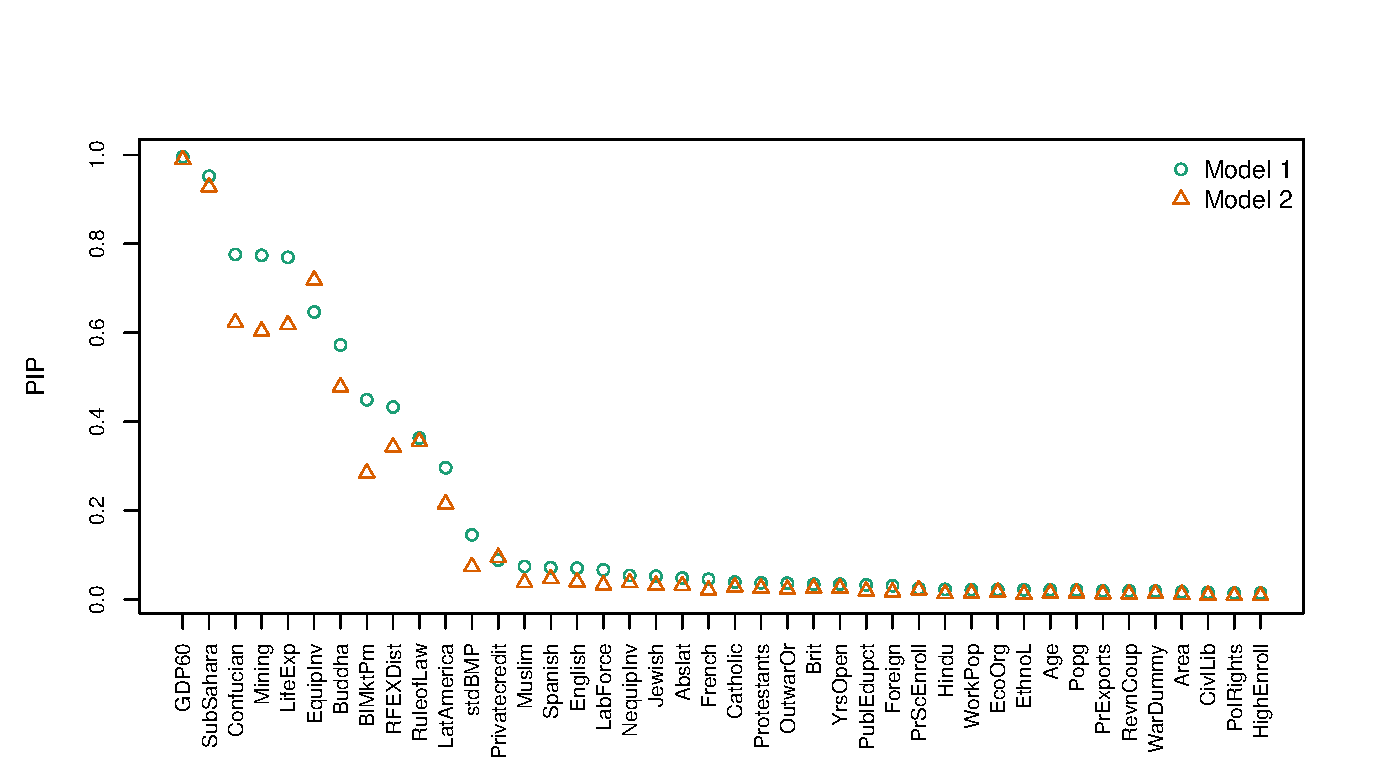
\includegraphics[width=\linewidth]{Figures/ch2/plotCompPC6011rnd}
		\begin{minipage}{0.8\textwidth}
			\footnotesize
			\emph{Note: Model 1=hyper-g, random model prior; Model 2=\ac{UIP}, random model prior}
		  \end{minipage}
\end{figure}
%

\section{Jointness of financial indicators}\label{ch2app:joint}
To check the dependence between our financial variables, we compute the so--called jointness measure, which is based on the posterior distributions of explanatory variables over the model space. The goal of this exercise is to determine whether the different financial variables capture different sources of information in explaining the dependent variable (jointness) or if they represent similar factors and should not be considered jointly in the model (disjointness) \parencite{leysteel2007}.

Jointness statistics for our financial indicators are available in Tables \ref{ch2tab:joint1}--\ref{ch2tab:joint3} with each table representing a different approach to jointness computation. Tables \ref{ch2tab:joint1} and \ref{ch2tab:joint2} show that none of the numbers exceeds the threshold suggested by \textcite{leysteel2007} (LS) for decisive (dis)jointness. Nevertheless, jointness statistics for some of the pairs suggest very strong jointness (e.g. market capitalization and private credit). Another way of constructing jointness statistic has been developed by \textcite{doppelhoferweeks2009} (DW). Regarding DW statistic, we find strong substitutability for private credit and net interest margin. However, as has been stressed by \textcite{leysteel2009b}, DW jointness statistic may become very sensitive and volatile if one of the variables has high \ac{PIP} and the other has a very low one. This is indeed the situation we encounter in our analysis. In addition, if the net interest margin and private credit were to be strong substitutes in a sense they would represent very similar factors and thus be mutually replaceable in the estimation process, they should also exhibit the same importance regarding economic growth if considered separately. These findings make us believe that the LS statistics are more appropriate to judge the interdependence between financial indicators.

\begin{table}[!htbp]
\caption{Financial indicators, jointness statistics according to \textcite{leysteel2007}}
\label{ch2tab:joint1}
\small
\centering
\begin{tabular}{llllll}
   \toprule
  Net interest margin & . & &  &  &  \\ 
  Bank Z-score & 0.335 & . & & & \\ 
  Private credit & 0.058 & 0.025 & . & &  \\ 
  Market capitalization & 0.025 & 0.014 & 0.011 & . & \\ 
  Market turnover & 0.224 & 0.158 & 0.041 & 0.027 & . \\ 
   \bottomrule
\end{tabular}
\end{table}

\begin{table}[!htbp]
\caption{Financial indicators, jointness statistic according to \textcite{leysteel2007}, alternative}
\label{ch2tab:joint2}
\small
\centering
\begin{tabular}{llllll}
   \toprule
  Net interest margin & . &  &  &  &  \\ 
  Bank Z-score & 0.251 & . &  &  &  \\ 
  Private credit & 0.055 & 0.024 & . &  &  \\ 
  Market capitalization & 0.024 & 0.013 & 0.011 & . &  \\ 
  Market turnover & 0.183 & 0.136 & 0.039 & 0.027 & . \\ 
   \bottomrule
\end{tabular}
\end{table}

\begin{table}[!htbp]
\caption{Financial indicators, jointness statistic according to \textcite{doppelhoferweeks2009}}
\label{ch2tab:joint3}
\small
\centering
\begin{tabular}{llllll}
   \toprule
  Net interest margin & . &  &  & & \\ 
  Bank Z-score & -0.372 & . &  &  & \\ 
  Private credit & \textbf{-2.373} & -1.025 & . &  & \\ 
  Market capitalization & 0.028 & -0.645 & -0.521 & . & \\ 
  Market turnover & -0.829 & 0.165 & -0.331 & 0.256 & . \\ 
   \bottomrule
\end{tabular}
\end{table}  
%

\begin{table}[!ht] \centering 
	\caption{First-stage regression, 2SLS--BMA}
	\label{app1tab:1ststageIV} 
  \begin{tabular}{@{\extracolsep{5pt}}lc}
  \\[-1.8ex]\hline
  \hline \\[-1.8ex] 
   & \multicolumn{1}{c}{\textit{Dependent variable:}} \\ 
  \cline{2-2}
  \\[-1.8ex] & Net interest margin \\
  \hline \\[-1.8ex]
   Latitude & $-$0.054$^{***}$ \\
	& (0.017) \\ 
   Years open & $-$1.851$^{*}$ \\
	& (1.012) \\ 
   Rule of law & $-$2.086$^{**}$ \\
	& (1.036) \\
   Crises tally & 3.290$^{***}$ \\ 
	& (0.769) \\ 
  \hline \\[-1.8ex]
  Observations & 60 \\
  R$^{2}$ & 0.730 \\
  Adjusted R$^{2}$ & 0.711 \\ 
  Residual Std. Error & 1.748 (df = 55) \\ 
  F Statistic & 37.206$^{***}$ (df = 4; 55) \\ 
  \hline
  \hline \\[-1.8ex]
  \textit{Note:}  & \multicolumn{1}{r}{$^{*}$p$<$0.1; $^{**}$p$<$0.05; $^{***}$p$<$0.01} \\
  \end{tabular}
  \end{table}

\end{subappendices}
\end{refsection}